\documentclass[10pt]{article}

\newcommand\hmmax{0}
\newcommand\bmmax{2}
\usepackage{amsthm, amsmath,amssymb,bbm}
\DeclareMathAlphabet{\mathbbm}{U}{bbm}{m}{n}
\usepackage{natbib}
\usepackage{multirow}
\usepackage{subfigure}
\usepackage{makecell}
\usepackage{booktabs}
\usepackage{array}
\usepackage{tabularx}
\usepackage{tabulary}
\usepackage{caption}
\usepackage{booktabs}
\usepackage{url}
\usepackage{algorithm}
\usepackage{algpseudocode}
\usepackage{bm}
\usepackage{wrapfig}
\usepackage{lipsum}
\usepackage{mathrsfs}
\usepackage{dsfont}
\usepackage{titling}
%\usepackage{txfonts}
\usepackage{relsize}
\usepackage{enumitem}
\usepackage{setspace}
\usepackage[colorlinks,
linkcolor=tpurple,
anchorcolor=tpurple,
citecolor=tpurple
]{hyperref}

\usepackage{tikz}
\usetikzlibrary{positioning}

% arxiv 
\usepackage[nameinlink,capitalize]{cleveref}
% journal
%\usepackage[capitalize]{cleveref}

%%%%%%% Setup of User-Defined Colors

\definecolor{myred}{HTML}{ae1908}
\definecolor{myblue}{HTML}{05348b}
\definecolor{myorange}{HTML}{ec813b}
\definecolor{mylightblue}{HTML}{9acdc4}
\definecolor{tpurple}{HTML}{743096}
\definecolor{myyellow}{HTML}{e5a84b}
\definecolor{mygreen}{HTML}{6bb392}

\definecolor{revisecolor}{HTML}{000000}



%%%%%%% Setup of Colorlinks, Margin, Textwidth, Font, Numbering ...

%\setstretch{2}
%\usepackage{geometry}
% \geometry{
% a4paper,
 %total={170mm,257mm},
% left=28mm,
% top=30mm,
% }
\textwidth=6in
\usepackage{fullpage}
%\setstretch{2}

% caption size
\usepackage[font={footnotesize,it}]{caption}

\numberwithin{equation}{section}


%%%%%%% My macros
\usepackage{smile}
\newcommand{\indep}{\perp \!\!\! \perp}
\newcommand*{\supp}{\mathrm{supp}}
\usepackage{etoolbox}
\newtoggle{vaos}
\togglefalse{vaos}
\newcommand{\aosversion}[2]{\iftoggle{vaos}{#1}{#2}}

% Definition of Roman Numbers
\newcommand{\Rom}[1]{\text{\uppercase\expandafter{\romannumeral #1\relax}}}
\newcommand{\todo}[1]{{\color{tpurple} \colorbox{tpurple!30}{Todo} #1}}
\newcommand{\question}[1]{{\color{tpurple} \colorbox{tpurple!30}{Question} #1}}
\newcommand{\red}[1]{{\color{red} #1}}
\newcommand{\blue}[1]{{\color{blue} #1}}


\newcommand{\myred}[1]{{\color{myred} #1}}
\newcommand{\myblue}[1]{{\color{myblue} #1}}
\newcommand{\mylightblue}[1]{{\color{mylightblue} #1}}
\newcommand{\myorange}[1]{{\color{myorange} #1}}
\newcommand{\mypurple}[1]{{\color{mypurple} #1}}
\newcommand{\myyellow}[1]{{\color{myyellow} #1}}
\newcommand{\mygreen}[1]{{\color{mygreen} #1}}

\def\r#1{\textcolor{red}{\bf #1}}
\def\b#1{\textcolor{blue}{\bf #1}}
\begin{document}
\setcounter{tocdepth}{2}

\title{Environment Invariant Linear Least Squares}
\author{ 
	Jianqing Fan
	\qquad Cong Fang
	\qquad Yihong Gu
	\qquad Tong Zhang}
\date{Princeton University, Peking University, and \\ The Hong Kong University of Science and Technology}
\maketitle

\begin{abstract}
\setstretch{1}
    This paper considers a multi-environment linear regression model in which data from multiple experimental settings are collected. The joint distribution of the response variable and covariates may vary across different environments, yet the conditional expectations of the response variable, given the unknown set of important variables, are invariant. Such a statistical model is related to the problem of endogeneity, causal inference, and transfer learning. The motivation behind it is illustrated by how the goals of prediction and attribution are inherent in estimating the true parameter and the important variable set. We construct a novel {\it environment invariant linear least squares (EILLS)} objective function, a multi-environment version of linear least squares regression that leverages the above conditional expectation invariance structure and heterogeneity among different environments to determine the true parameter. Our proposed method is applicable without any additional structural knowledge and can identify the true parameter under a near-minimal identification condition related to the heterogeneity of the environments. We establish non-asymptotic $\ell_2$ error bounds on the estimation error for the EILLS estimator in the presence of spurious variables. Moreover, we further show that the $\ell_0$ penalized EILLS estimator can achieve variable selection consistency in high-dimensional regimes. These non-asymptotic results demonstrate the sample efficiency of the EILLS estimator and its capability to circumvent the curse of endogeneity in an algorithmic manner without any additional prior structural knowledge.  To the best of our knowledge, this paper is the first to realize statistically efficient invariance learning in the general linear model.
\end{abstract} 
\noindent{\bf Keywords}: Least Squares, Endogeneity, Multiple Environments, Invariance, Heterogeneity, Structural Causal Model, Invariant Risk Minimization.
{

% BEGIN INCLUDED SOURCE: tex/main_text.tex
\section{Introduction}

The development of statistical regression methods dates back to the least squares proposed in the early nineteenth century \citep{legendre1805leastsquares, gauss1809leastsquares}. The ordinary linear least squares method, also known as {\it the combination of observations}, uses observations (data) to fit a model predicting the {\it response variable} as a linear function of several designated {\it explanatory variables}. At that time, the fitted models for specific tasks, for example, determining lunar motion, were successfully deployed in the real world for predicting the unseen future and were of great commercial and military significance \citep{stigler1986history}. For example, such a prediction of lunar liberation helps determine the ship's position and facilitates navigating the ocean during the Age of Discovery. This kind of prediction requires only a strong correlation with the response variable. Since then, one ultimate goal of fitting a regression model is to discover the law, which is {\it invariant} across time and space or more broadly {\it environments} to some extent, from the data and then ground it in the real world for prediction. The latter requires understanding causation.  

With the rapidly growing amount of high-dimension data in the era of big data, there is a surge in demand for making predictions based on numerous explanatory variables \citep{fan2014challenges,  wainwright2019high, fan2020statistical}. Compared to the circumstances in the nineteenth century, in which the target is to predict the response variable using fixed, carefully chosen explanatory variables, we are now in the stage where the algorithms such as Lasso \citep{tibshirani1997lasso}, SCAD \citep{fan2001variable}, Dantzig selector \citep{candes2007dantzig}, to name a few, can automatically select tens of important variables responsible for the response variable out of thousands or more of candidates. There is considerable literature on the theoretical analysis of these methods regarding the estimation error and variable selection property \citep{zhao2006model, candes2007dantzig, bickel2009simultaneous, buhlmann2011statistics, wainwright2019high, fan2020statistical}, demonstrating their successes and promising prospects.

Let us use a thought experiment to illustrate the underlying risks and potential remedies when incorporating more candidate variables. Suppose our task is to fit a model to classify cows and camels based on extracted hierarchical features from some ``oracle'' agent. We find a dataset $\mathcal{D}$ containing 10k images of cows and camels from the Internet and use 70\% of them to train a classifier on top of two features provided by the agent: the back shape $x_1$, and the background color $x_2$. It is contemplated that cows often appear on the grass while most camels appear on the sand. This indicates that we can use $x_2$ to build a classifier that works well on the training data and the remaining $30\%$ test data by classifying whether the background color is green or yellow. Moreover, incorporating $x_2$ can also increase the accuracy of the classifier built on $x_1$. However, introducing $x_2$ is not what we expected: it may result in a disaster when we deploy it in real-world applications, for example, a detector in a place farming camels and cows, in which the background color is fixed. Problems of a similar nature arise readily in realistic applications \citep{torralba2011unbiased, geirhos2020shortcut} and easily in high dimensions \citep{fan2014endogeneity}. A natural question is whether there are any purely data-driven methods to address such an endogeneity problem. Consider the case where we have another dataset $\tilde{\mathcal{D}}$ in which an association between the background color and object label still exists yet slightly perturbs; for example, 60\%/90\% of the camels stand on sand in the two datasets, respectively. Intuitively, we can combine two different associations between the background color and the object label in these two datasets and infer that $x_2$ may be a ``spurious'' variable for prediction or causation.

The above thought experiment demonstrates that we may suffer from the ``curse of endogeneity'', that the conditional expectation of the response given all the explanatory variables may diverge from the law of interests, when including a lot of variables besides the true important variables before estimation \citep{fan2014challenges}. Such a problem will deviate our route toward building a decent prediction model grounded in the real world and yield non-robust predictions in other environments. Meanwhile, a potential data-driven strategy is to utilize the \emph{heterogeneity} across datasets. This paper implements the above intuition to the linear regression model in statistical modeling, methodology, and theory. We propose a multi-environment version of linear least squares, whose key idea can be summarized as \emph{the combination of combinations of observations} under heterogeneous environments: it combines the linear least squares (\emph{combination of observations}) solutions across different datasets and uses their differences to determine the true parameter $\bbeta^*$ in a completely data-driven manner.

\subsection{The Problem under Study}

In this work, we are interested in predicting the response variable $y \in \mathbb{R}$ with a linear function of the explanatory variable $\bx \in \mathbb{R}^p$ using data from \emph{multiple environments}. Suppose we have collected data from multiple resources/environments. Let $\mathcal{E}$ be the set of environments. For each \emph{environment} $e\in \mathcal{E}$, we observe $n$ i.i.d. $(\bx_1^{(e)}, y_1^{(e)}), \ldots, (\bx_n^{(e)}, y^{(e)}_n) \sim \mu^{(e)}$, typically assumed from the linear model\footnote{Our main theoretical results still hold if the conditional expectation is replaced by $\mathbb{E}[\varepsilon^{(e)} \bx_{S^*}^{(e)}]=0$, in which $\bbeta^*$ is the best linear predictor on important variables.}
\begin{align}
\label{eq:intro-dgp}
    y^{(e)} = (\bbeta^*_{S^*})^\top \bx_{S^*}^{(e)} + \varepsilon^{(e)} ~~~~~ \text{with} ~~~~ \mathbb{E}[\varepsilon^{(e)}|\bx_{S^*}^{(e)}] \equiv 0,
\end{align} where the unknown set of important variables $S^* = \{j: \beta_j^* \neq 0\}$ and the model parameters $\bbeta^*$ are the same, or \emph{invariant}, across different environments, while $\mu^{(e)}$, the distribution of $(\bx^{(e)},y^{(e)})$, may vary. We aim to estimate $\bbeta^*$ and $S^*$ using the $n\cdot |\mathcal{E}|$ data $\{(\bx_i^{(e)}, y_i^{(e)})\}_{e\in \mathcal{E}, i\in \{1,\ldots, n\}}$. The model assumptions of multiple environments resemble and slightly relax the assumptions in this paper's predecessors, for example, \cite{peters2016causal, rojas2018invariant, pfister2021stabilizing, yin2021optimization}.

The main challenge behind identifying $\bbeta^*$ is that the exogeneity condition \citep{engle1983exogeneity} on all predictors, i.e., $\mathbb{E}[\varepsilon^{(e)}|\bx^{(e)}] \equiv 0$ or at least $\mathbb{E}[\varepsilon^{(e)} \bx^{(e)}] = 0$, no longer holds for each single $e\in \mathcal{E}$.  This arises easily in the high-dimensional settings as argued in \cite{fan2014endogeneity} and \cite{fan2014challenges} where a different data-driven strategy is proposed to solve the problem. Instead, for each environment $e\in \mathcal{E}$, the exogeneity condition only holds on the important variables according to \eqref{eq:intro-dgp}. The only assumption available now is
\begin{align}
\label{eq:intro-invariance}
    \forall e\in \mathcal{E}, ~~~~~~ \mathbb{E}[y^{(e)}|\bx^{(e)}_{S^*}] = (\bbeta^*_{S^*})^\top \bx^{(e)}_{S^*},
\end{align} while $\mathbb{E}[y^{(e)}|\bx^{(e)}]$ is not necessarily equal to $(\bbeta^*)^\top \bx^{(e)}$ for each single environment $e\in \mathcal{E}$. This further indicates that $\bbeta^*$ may not be the best linear predictor for environment $e\in \mathcal{E}$, and the gap can be potentially large. Recall when the covariance matrix $\mathbb{E}[\bx^{(e)} (\bx^{(e)})^\top]$ is positive definite, the best linear predictor for environment $e\in \mathcal{E}$ can be written as
\begin{align}
\label{eq:intro-lse-sol}
    \bbeta^{(e)} = \bbeta^* + \left(\mathbb{E}[\bx^{(e)} (\bx^{(e)})^\top]\right)^{-1} \mathbb{E}[\bx^{(e)} \varepsilon^{(e)}].
\end{align} This implies that when only one environment $e\in \mathcal{E}$ is taken into consideration, one can obtain a reduced mean squared error by incorporating those \emph{linear spurious variables}, defined as the variables $x_j$ satisfying $\mathbb{E}[x_j^{(e)} \varepsilon^{(e)}]\neq 0$, and other variables correlated to these variables. They help predict $ \varepsilon^{(e)}$ and reduce prediction error under this environment.   An example is the variable measuring ``background color'' in the above thought experiment. However, these variables are unstable because the corresponding association between these variables and $y$ may vary or even be adversarial in other or unseen environments, leading to biased predictions.

Two ultimate goals of fitting a statistical model using data are prediction and attribution. Regarding ``prediction'', we hope our fitted model can make decent predictions on unseen data grounded in the real world rather than only on the ``demo'' test data. Regarding ``attribution'' \citep{efron2020prediction}, we wish to attribute the outcome/response variable to the significant variables of the fitted model such that the fitted model can lead to true scientific claims. See also Chapter 1 of \cite{fan2020statistical}. We illustrate that the goal of estimating $\bbeta^*$ and $S^*$ for the model \eqref{eq:intro-dgp} unifies the above two seemingly separate goals, thereby expounding the motivation and importance of the multi-environment linear regression model.

\noindent \textbf{Prediction.} Consider the case where the potential distribution of the unseen data $\tilde{\mu}$ may be different from those $\{\mu^{(e)}\}_{e\in \mathcal{E}}$ yet shares the same conditional expectation structure $\mathbb{E}_{\tilde{\mu}}[y|\bx_{S^*}] = (\bbeta^*_{S^*})^\top \bx_{S^*}$ as those of observations in \eqref{eq:intro-dgp}. Without informing of the unseen data distribution ahead, we can define the out-of-sample $L_2$ risk in an adversarial manner as
\begin{align*}
    \mathsf{R}_{\mathtt{oos}}(\bbeta) = \sup_{\substack{\mathbb{E}_\mu[y|\bx_{S^*}] = (\bbeta^*_{S^*})^\top \bx_{S^*} \\ \mathrm{Var}_{\mu}[y|\bx_{S^*}] \lor \max_{1\le j\le p}\mathbb{E}_{\mu}[x_j^2] \le \sigma^2}}  \mathbb{E}_{\mu}\left[|\bbeta^\top \bx - y|^2\right].
\end{align*} 
It follows from \cref{prop:oos-definition-property} in \cref{subsec:problem-formulation} that $\bbeta^*$ minimizes $\mathsf{R}_{\mathtt{oos}}(\bbeta)$ though it may not be the best linear predictor for a specific environment $\tilde{\mu}$. This demonstrates that $\bbeta^*$ is the optimal linear predictor robust to all potential distribution shifts on the unseen data to some extent. Moreover, \cref{prop:oos-definition-property} also implies that the $\ell_2$ error $\|\bbeta - \bbeta^*\|_2$ can be treated as an surrogate of the excess out-of-sample $L_2$ risk. This connects the estimation error of $\bbeta^*$ to the ``adversarial'' mean squared error on potential unseen data.

\noindent \textbf{Attribution.} Let us restrict the multi-environment linear regression model to a specific instance -- data with different experimental settings \citep{didelez2012direct, peters2016causal} in the context of causal inference. To be specific, suppose there exists an environment $e_0\in \mathcal{E}$ with observational data, and the rest are environments with interventional data \citep{he2008active}, in which some interventions are performed on the variables other than the response variable $y$. The distribution of the variables in each environment can be encoded as a Structural Causal Model (SCM) \citep{glymour2016causal}. Under the modularity \citep{scholkopf2012causal} assumption for SCMs that the intervention on variable $x_j$ only changes the distribution of $\mathbb{P}(x_j|\bx_\mathsf{pa(j)})$ where $\mathsf{pa}(j)$ is the set of direct causes of $x_j$, we can see that $S^*$ in this instance is exactly the ``direct cause'' of the response variable. In this case, inferring $S^*$ from data coincides with discovering the direct cause of the variable $y$, while estimating $\bbeta^*$ is exactly estimating the true causal coefficients characterizing the mechanism $\mathbb{P}(y|\bx_{\mathsf{pa(y)}})=\mathbb{P}(y|\bx_{S^*})$.  See \cref{subsec:causal} for additional details.

\subsection{Related Works}

Multi-environment regression is common in many applications \citep{meinshausen2016methods, vcuklina2021diagnostics}. There is considerable literature proposing methods to estimate $\bbeta^*$ and $S^*$ starting from the pioneering work of \cite{peters2016causal}, in which they propose the ``Invariant Causal Prediction'' (ICP) to do causal discovery. The key idea behind it is the modularity assumption of SCMs, which is also referred to as invariance, autonomy \citep{haavelmo1944probability, aldrich1989autonomy}, and stability \citep{dawid2010identifying}. To be specific, \cite{peters2016causal} considers the multiple environments setting, in which the intervention may be applied to unknown variables other than $y$, leading to the following multi-environment linear regression model,
\begin{align}
\label{eq:intro-icp-cond}
    y^{(e)} = (\bbeta^*)^\top\bx^{(e)} + \varepsilon^{(e)} ~~~~~ \text{with} ~~~~~ \varepsilon^{(e)} \sim \mu_\varepsilon, ~\varepsilon^{(e)} \indep \bx_{S^*}^{(e)}, ~\text{and}~\mathbb{E}[\varepsilon^{(e)}]=0.
\end{align} They exploit the conditional distribution invariance structure, i.e., $\varepsilon^{(e)}|\bx_{S^*}^{(e)}$, and propose a hypothesis testing procedure which can guarantee the selected set $\hat{S}$ satisfies $\mathbb{P}(\hat{S} \subseteq S^*) \ge 1-\alpha$ for given Type-I error $\alpha>0$. There is considerable literature extending this idea to other models such as \cite{heinze2018invariant, pfister2019invariant}. Though the Type-I error is guaranteed for their method, these procedures may collapse to conservative solutions, such as $\hat{S}=\emptyset$, and there is a lack of guarantee in the power of the test.

The conservative nature of ICP methods has sparked the development of numerous optimization-based methods. Built upon the invariance principle, there is also considerable literature \citep{ghassami2017learning, rothenhausler2019causal, rothenhausler2021anchor} proposing provably sample-efficient regression methods for estimating the causal parameter $\bbeta^*$. However, they rely on additional, restrictive structures that simplify the original problem considerably. For instance, the Causal Dantzig \citep{rothenhausler2019causal} presumes a linear SCM model with the heterogeneity of environments resulting from additive interventions. Implementing these methods in practical scenarios necessitates expert domain knowledge to validate these structures before estimation. This requirement introduces potential risks of model misspecification, as these methods are specifically tailored to the assumed structures.

There is also a considerable literature designing methods for the generic linear model \eqref{eq:intro-icp-cond}, for example, \cite{ rojas2018invariant, pfister2021stabilizing, yin2021optimization}. However, these methods tend to be heuristic, and finite sample guarantees are lacking. Inspired by the goal of achieving out-of-distribution generalization, \cite{arjovsky2019invariant} introduced another heuristic and model-agnostic approach. Their method, Invariant Risk Minimization (IRM), seeks a data representation such that the optimal predictors based on it are invariant across all environments. The ideas of IRM and its variants are widely applied in many machine learning tasks \citep{sagawa2019distributionally, zhang2020invariant, krueger2021out, lu2021nonlinear}. Nevertheless, the theoretical understanding of invariance learning remains sparse, and the performance improvement of these methods over the standard empirical risk minimization is not clear \citep{rosenfeld2020risks, kamath2021does}. 

Another critical issue associated with these invariance learning methods is the inadequacy of theoretical insights into their identification conditions, which characterizes when it is possible to identify $\bbeta^*$ in the model \eqref{eq:intro-icp-cond} using infinite data from {\it finite} environments. While \cite{peters2016causal} delves into this issue, providing sufficient conditions for specific intervention and SCM structure types, it falls short of offering general criteria. Similarly, \cite{arjovsky2019invariant} also has some preliminary discussions on linear models, yet it stipulates an impractical requirement: $|\mathcal{E}| \ge d$. The understanding of the identification condition for a developed method is of great significance because it elucidates the method's sample efficiency in terms of the number of environments $|\mathcal{E}|$ required: a stronger identification condition may necessitate a potentially increased number of environments $|\mathcal{E}|$ to recover $\bbeta^*$.

It is worth noting that the invariance structure we can exploit depends on the perturbations we expect in real-world scenarios. Due to its clear causal interpretation, the idea of invariance is also widely adopted in domain adaptation, transfer learning, and out-of-distribution generalization. Numerous invariance forms have been proposed based on various expected perturbations beyond the residual invariance \eqref{eq:intro-dgp}. There is also considerable literature designing methods to leverage these invariance structures \citep{muandet2013domain, gong2016domain, heinze2021conditional} using data from multiple environments. A notable example in classification tasks is the invariance of the label conditional distribution, expressed as $\mathbb{P}^{(e)}(\phi(\bx)|y)\equiv q(\bx, y)$, where $\phi(\cdot)$ is an unknown data representation. We refer readers to \cite{chen2021domain, wang2023causal} for an overview.


\subsection{New Contributions and Comparison with Predecessors}

The significance of recovering $S^*$ and $\bbeta^*$ in the model \eqref{eq:intro-dgp}, the sample inefficiency of previous methods in terms of $n$ and $|\mathcal{E}|$, and the lack of theoretical understanding in invariance learning raise the following question:
\begin{align*}
    \begin{split}
    &\text{\it Is provably sample-efficient estimation of $\bbeta^*$ and $S^*$ in the model \eqref{eq:intro-dgp}}\\
    &\text{\it possible under a general, minimal identification condition?} \\
    \end{split}
\end{align*}

This paper provides an affirmative ``yes'' to the above question. In this paper, we propose the \emph{environment invariant linear least squares (EILLS)} estimator that regularizes linear least squares with a \emph{focused linear invariance regularizer} which promotes the invariance or exogeneity on selected variables. In particular, the population-level EILLS objective over the environments $\mathcal{E}$ is defined as
\begin{align}
\label{eq:intro-eills-obj-popu}
    \mathsf{Q}_\gamma(\bbeta) = \underbrace{\sum_{e\in \mathcal{E}} \mathbb{E} \left[|y^{(e)} - \bbeta^\top \bx^{(e)}|^2\right]}_{\mathsf{R}(\bbeta)} + \gamma \underbrace{\sum_{j=1}^p \mathds{1}\{\beta_j\neq 0\} \times  \sum_{e\in \mathcal{E}} \left|\mathbb{E} [(y^{(e)} - \bbeta^\top \bx^{(e)}) x_j^{(e)}]\right|^2 }_{\mathsf{J}(\bbeta)}
\end{align} with some hyper-parameter $\gamma>0$. From a high-level viewpoint, the introduction of the regularizer $\mathsf{J}(\cdot)$ leverages the invariance structure \eqref{eq:intro-invariance} while the sum of $L_2$ loss $\mathsf{R}(\cdot)$ requires a good overall solution and prevents it from collapsing to conservative solutions such as $\bbeta=0$.  See also \cite{fan2014endogeneity} for a similar method to deal with endogeneity in high-dimensional regression. To get a crude sense of what $\mathsf{J}(\cdot)$ imposes, note that $\mathsf{J}(\cdot)$ discourages selecting variables that have a strong correlation with the fitted residuals in some environments and hence encourages the selected variables to be exogenous, uncorrelated with the fitted residuals for all the environments in a sense that
\begin{align*}
    \forall e\in \mathcal{E}, j~\text{with}~\bar{\beta}_j\neq 0 ~~~~~~~~ \mathbb{E} [(y^{(e)} - \bar{\bbeta}^\top \bx^{(e)}) x_j^{(e)}] = 0.
\end{align*} 
This can be seen when $\gamma \to \infty$ and has a similar spirit of imposing $\mathbb{E}\big[y^{(e)} |\bx_{\supp(\bar{\bbeta})}^{(e)}\big]=\bar{\bbeta}^\top \bx^{(e)}$ for all the $e\in \mathcal{E}$. As for the empirical counterpart, given the $n \cdot |\mathcal{E}|$ observations from $|\mathcal{E}|$ environments, the EILLS estimator minimizes $\hat{\mathsf{Q}}_\gamma(\bbeta)$
which substitutes all the expectations in \eqref{eq:intro-eills-obj-popu} by their corresponding empirical means. One can also use the EILLS estimator in high-dimensional case ($p>n$) by adding an $\ell_0$ penalty with some pre-defined hyper-parameter $\lambda>0$ when needed.

We further develop theories in \cref{sec:theory} characterizing when our proposed EILLS estimator can consistently estimate $\bbeta^*$ and $S^*$. We show that our EILLS estimator can identify $\bbeta^*$ with some large enough $\gamma$ in the sense that $\bbeta^*$ is the unique minimizer of the population-level objective \eqref{eq:intro-eills-obj-popu} if
\begin{align}
\label{eq:intro-ident}
    \forall S\subseteq \{1,\ldots, p\} ~\text{with}~ \sum_{e\in\mathcal{E}} \mathbb{E}[\varepsilon^{(e)} \bx^{(e)}_S] \neq 0 ~~~ \implies ~~~\exists e, e'\in \mathcal{E}, ~~\bbeta^{(e,S)} \neq \bbeta^{(e',S)}
\end{align} where $\bbeta^{(e,S)} = \argmin_{\supp(\bbeta) \subseteq S} \mathbb{E}[|y^{(e)} - \bbeta^\top \bx^{(e)}|^2]$ is the best linear predictor constrained on $S$ for environment $e\in \mathcal{E}$. Such a general identification condition is minimal if only linear information is used. This demonstrates that the EILLS objective can automatically circumvent the problem caused by endogeneity if incorporating any {\it pooled linear spurious variable}, defined as the variable $x_j$ satisfying $\sum_{e\in\mathcal{E}} \mathbb{E}[\varepsilon^{(e)} x^{(e)}_j] \neq 0$, will lead to shifts in the least squares solutions among different environments, and it is sample-efficient in terms of $|\mathcal{E}|$ required. 

Under the general identification condition \eqref{eq:intro-ident}, a series of non-asymptotic results are presented for the EILLS estimator when $\gamma$ is greater than some critical threshold $\gamma_*$, illustrating the sample efficiency of our proposed EILLS estimator. In the low-dimensional regime, the vanilla EILLS estimator can obtain the optimal rate for linear regression. Moreover, the EILLS objective also embodies a variable selection property that can eliminate all the linear spurious variables while keeping all the true important variables provided $n$ is large enough. In the high-dimensional regime where $p > n$, the $\ell_0$ regularized EILLS estimator can achieve the variable selection consistency $\{j: \hat{\beta}_{j} \neq 0\} = S^*$ with high probability in a similar manner to the standard $\ell_0$ regularized least squares. Non-asymptotic upper bounds on $\gamma_*$ for some concrete models are calculated, illustrating the applicability of our general result. 

This paper proposes a provably sample-efficient estimation method for the general model \eqref{eq:intro-dgp}. To the best of our knowledge, it is the {\it first} estimator with non-asymptotic guarantees in terms of $|\mathcal{E}|$ and $n$ for the general multi-environment linear regression model \eqref{eq:intro-dgp}, or a slightly restricted version of it, e.g., \eqref{eq:intro-icp-cond}. As a comparison, previous provably sample-efficient estimation methods, like anchor regression \citep{rothenhausler2021anchor} and Causal Dantzig \citep{rothenhausler2019causal}, have predominantly been confined to the linear SCM with additive intervention case, that is, $((\bx^{(e)})^\top, y^{(e)})^\top \gets \bB ((\bx^{(e)})^\top, y^{(e)})^\top + g(\ba^{(e)}, \bvarepsilon^{(e)})$ with some invariant matrix $\bB\in \mathbb{R}^{(p+1)\times (p+1)}$. These imposed structures not only restrict the scalable applicability of these methods in practice but also hinder their potential for extension to nonlinear models. While our method primarily addresses the linear model, it demonstrates promise for extension to nonlinear models; see a discussion in \cref{sec:ex-nonlinear}. Our approach also shares a similar spirit to the ICP method but necessitates a weaker identification condition to recover the true parameter $\bbeta^*$. This implies that our method is more sample-efficient than ICP regarding $|\mathcal{E}|$. Furthermore, we conduct a numerical analysis to benchmark our proposed EILLS estimator against various other invariance methods, demonstrating its superior performance in \cref{sec:simulation}.


\section{Setup and Background}
\label{sec:setup}

\subsection{Multi-Environment Linear Regression}
\label{subsec:problem-formulation}

Suppose we are interested in uncovering the ``scientific truth'' between the response variable $y$ and $\bx_{S^*}$, a sub-vector of $p$-dimensional covariate vector $\bx \in \mathbb{R}^p$. As $S^*$ is unknown, we collect many more variables, but the collected covariates are easily correlated with residuals of $y$ on $\bx_{S^*}$ \citep{fan2014endogeneity, fan2014challenges}. This gives rise to the following more realistic assumption: The distribution of $\bx$ and $y$, $\mu$, satisfies
\begin{align}
\label{eq:true-law-set}
    \mu \in \mathcal{U}_{\bbeta^*, \sigma^2} = \Bigg\{\begin{split}\mu&: ~\mathbb{E}_\mu[y|\bx_{S^*} ] = (\bbeta^*_{S^*})^\top \bx_{S^*}, \text{Var}_{\mu}[y|\bx_{S^*}] \le \sigma^2, ~~ \mu\text{-a.s.} ~ \bx, \\
    &~~~~~\forall j \in [p], ~ \mathbb{E}_{\mu}[x_j^2] \le \sigma^2
    \end{split}
    \Bigg\}.
\end{align} Here, $S^* \subseteq [p]$ denotes the set of important variables that contribute to explain the ``truth'',  $\bbeta^*$ is the parameter of interest whose support set $\supp(\bbeta^*)$ is $S^*$, and $\sigma^2$ is any given positive number.

With only one environment, it is impossible to identify $S^*$.
Consider the data collected from multiple environments: in each environment $e$, the data $(\bx^{(e)}, y^{(e)})$ follows from some law $\mu^{(e)}$ in $\mathcal{U}_{\bbeta^*, \sigma^2}$. Denote the set of environments by $\mathcal{E}$. For each environment $e\in \mathcal{E}$, we observe $n^{(e)}$ i.i.d. samples $(\bx^{(e)}_1,y^{(e)}_1),\ldots, (\bx^{(e)}_{n^{(e)}}, y^{(e)}_{n^{(e)}})  \sim \mu^{(e)}$ with $\mu^{(e)} \in \mathcal{U}_{\bbeta^*, \sigma^2}$. Let $\mathcal{D}^{(e)} = \{(\bx_i^{(e)}, y_i^{(e)})\}_{i=1}^{n^{(e)}}$ be the data collected from environment $e$. Our goal is to use the data $\{\mathcal{D}^{(e)}\}_{e\in \mathcal{E}}$ collected from multiple environments to find a linear predictor $f(\bx) = \bbeta^\top \bx$ that  minimizes the out-of-sample $L_2$ risk that is robust to all potential out-of-sample distributions in $\mathcal{U}_{\bbeta^*, \sigma^2}$. That is, find the minimizer of
\begin{align}
\label{eq:oos-mse}
    \mathsf{R}_{\mathtt{oos}}(\bbeta;\mathcal{U}_{\bbeta^*, \sigma^2}) = \sup_{\mu \in \mathcal{U}_{\bbeta^*, \sigma^2}} \mathbb{E}_{(\bx,y)\sim \mu} \left[ |y - \bbeta^\top \bx|^2 \right].
\end{align}
The following proposition asserts that $\bbeta^*$ is the unique minimizer of \eqref{eq:oos-mse}, whose proof is given in \aosversion{Appendix~\blue{B.1}}{\cref{prop:oos-definition-property-proof}}.

\begin{proposition}[Properties of $\mathsf{R}_{\mathtt{oos}}$] \label{prop:oos-definition-property} We have $\mathsf{R}_{\mathtt{oos}}(\bbeta^*;\mathcal{U}_{\bbeta^*, \sigma^2})=\sigma^2$, and for any $\bbeta \in \mathbb{R}^p$,
\begin{align}
\label{eq:optimal-beta-s-star}
\begin{split}
\sigma^2 \|\bbeta - \bbeta^*\|_2^2 \le \mathsf{R}_{\mathtt{oos}}(\bbeta;&\mathcal{U}_{\bbeta^*,\sigma^2}) - \mathsf{R}_{\mathtt{oos}}(\bbeta^*;\mathcal{U}_{\bbeta^*, \sigma^2}) \\
&\le \sigma^2 p^2 \|\bbeta-\bbeta^*\|_2^2 + 2 \sigma^2 p \|\bbeta_{[p]\setminus S^*}\|_2.
\end{split}
\end{align}
\end{proposition}
As a by-product, \cref{prop:oos-definition-property} also implies that $\|\bbeta - \bbeta^*\|_2$ can be seen as a surrogate metric for the out-of-sample $L_2$ risk \eqref{eq:oos-mse}. \cref{prop:oos-definition-property} motivates us to design methods to estimate the variable set $S^*$  and the true parameter $\bbeta^*$  using data from multiple environments $\mathcal{E}$ which share the same structure $\mathcal{U}_{\bbeta^*,\sigma^2}$. Particularly, define the CE-invariant set as follows. We will take advantage of the fact that $S^*$ is CE-invariant across $\mathcal{E}$.

\begin{definition}[CE-invariant Set] A variable set $S \subseteq [p]$ is \textbf{conditional expectation invariant} (CE-invariant) across environments $\mathcal{E}$ if there exists some $\bbeta$ with support set $S$ such that
\begin{align}
\label{eq:ce-invariant}
    \forall e\in \mathcal{E}, ~~~~~~ \mathbb{E} [y^{(e)}|\bx_{S}^{(e)}] = \bbeta_S^\top \bx_{S}^{(e)}.
\end{align}
\end{definition} 

\noindent \textbf{Necessity of heterogeneous environments. } The following proposition argues that introducing multiple environments, i.e., $|\mathcal{E}| \ge 2$, with potentially different distributions is necessary to identify $\bbeta^*$. The proof is given in \aosversion{Appendix~\blue{B.2}}{\cref{prop:necessary-multiple-envs-proof}}.

\begin{proposition} \label{prop:necessary-multiple-envs} Given fixed $\bbeta^*$, for any $\bbeta \in \mathbb{R}^p$ such that $\supp(\bbeta) \setminus S^* \neq \emptyset$, there exists some large enough $\sigma^2>0$ and $\mu \in \mathcal{U}_{\bbeta^*, \sigma^2}$ such that
\begin{align*}
    \mathbb{E}_{\mu}[y|\bx] = \bbeta^\top \bx.
\end{align*}
\end{proposition}

Note that $\mathbb{E} [|\mathbb{E}[y|\bx] - y|^2] \le \mathbb{E} [|f(\bx) - y|^2]$ for any measurable function $f$. Hence \cref{prop:necessary-multiple-envs} implies the population $L_2$ risk minimizer $f^{\mu} = \argmin_f \mathbb{E}_\mu [|f(\bx) - y|^2]$ for a specific $\mu$ is not necessarily equal to $f^*(\bx) = (\bbeta^*)^\top \bx$. Instead, the bias $\mathbb{E}[|(f^{\mu} - f^{*})(\bx)|^2]$ between the population $L_2$ risk minimizer and the true regression function $f^*$ can be arbitrarily large. It illustrates that running a linear regression on the data in one environment may not be able to estimate $\bbeta^*$ well. Instead, running a linear regression on data in one sole environment may introduce some \emph{spurious variables} even in a population aspect. These variables are spurious since incorporating them in the prediction model can increase the prediction performance in one environment. However, the associations between these variables and $y$ are unstable and can lead to much worse prediction performances in other environments.

To estimate $\bbeta^*$ well, we should use data from \emph{heterogeneous} environments and exploit the invariant structure \eqref{eq:ce-invariant}. This is the main idea of this paper: we will take advantage of the underlying heterogeneity and invariance to infer the important variable set $S^*$ and the true parameter $\bbeta^*$. Furthermore, we will show later in our theoretical analysis that only two environments, i.e., $|\mathcal{E}|=2$, are enough to estimate $\bbeta^*$ consistently.

\subsection{Notations}

The following notations will be used throughout this paper. Let $\mathbb{R}^+$ and $\mathbb{N}^+$ be the set of positive real numbers/integers, respectively. Let $|S|$ denote the cardinality of a set $S$. Define $2^S = \{A: A\subseteq S\}$. Denote by $[m]=\{1,\ldots, m\}$. Let $a\lor b = \max\{a,b\}$ and $a\land b = \min\{a,b\}$. We use $a(n) \lesssim b(n)$ or $a(n) = O(b(n))$ to represent that there exists some universal constant $C>0$ such that $a(n) \le C\cdot b(n)$ for all the $n \in \mathbb{N}^+$, and use $a(n) \gtrsim b(n)$ or $a(n) = \Omega(b(n))$ if $a(n) \ge c \cdot b(n)$ with some universal constant $c>0$ for any $n\in \mathbb{N}^+$. Denote $a(n) \asymp b(n)$ if $a(n) \lesssim b(n)$ and $a(n)\gtrsim b(n)$. We use the notations $a(n) \ll b(n)$, or $b(n) \gg a(n)$, or $a(n) = o(b(n))$ if $\limsup_{n\to\infty} (a(n) / b(n)) = 0$.

We use bold lower case letter $\bx = (x_1,\ldots, x_d)^\top$ to represent a $d$-dimension vector, let $\|\bx\|_q = (\sum_{i=1}^d |x_i|^q)^{1/q}$ be it's $\ell_q$ norm. We use $\supp(\bx) = \{j\in [d]: x_j \neq 0\}$ to denote the support set of the vector $\bx$. For any $S=\{j_1,\ldots, j_{|S|}\} \subseteq[d]$ with $j_1<j_2<\cdots<j_{|S|}$, we denote $[\bx]_{S} = (x_{j_1},\ldots, x_{j_{|S|}})^\top$ be the $|S|$-dimension sub-vector of $\bx$ and abbreviate it as $\bx_S$ when there is no ambiguity. We use bold upper case letter $\bA = [A_{i,j}]_{i\in [n], j\in [m]}$ to denote a matrix. Denote $\bA_{S,T} = [A_{i,j}]_{i\in S, j\in T}$ be the sub-matrix of $\bA$, and abbreviate $\bA_{S,S}$ as $\bA_S$. We let $\|\bA\|_2 = \max_{\bv\in \mathbb{R}^m, \|\bv\|_2=1} \|\bA \bv\|_2$.

For each $e\in \mathcal{E}$, suppose we have $n^{(e)}$ observations $\{(\bx_i^{(e)}, y_i^{(e)})\}_{i=1}^{n^{(e)}} \subseteq \mathbb{R}^p \times \mathbb{R}$ drawn i.i.d. from some distribution $\mu^{(e)}$. Let $\mathbb{E}[f(\bx^{(e)}, y^{(e)})] = \int f(\bx, y) \mu^{(e)}(d\bx, dy)$ and $\hat{\mathbb{E}}[f(\bx^{(e)},y^{(e)})] = \frac{1}{n^{(e)}} \sum_{i=1}^{n^{(e)}} f(\bx^{(e)}_i, y^{(e)}_i)$ for a measurable function $f$. Define the empirical $L_2$ risk $\hat{\mathsf{R}}^{(e)}$ and population $L_2$ risk $\mathsf{R}^{(e)}$  as
\begin{align}
\label{eq:def-l2-risk}
    \hat{\mathsf{R}}^{(e)}(\bbeta) = \hat{\mathbb{E}}\left[|y^{(e)} - \bbeta^\top \bx^{(e)}|^2\right] ~~~~ \text{and} ~~~~ \mathsf{R}^{(e)}(\bbeta) = \mathbb{E} \left[|y^{(e)} - \bbeta^\top \bx^{(e)}|^2\right].
\end{align} 
We also define $\varepsilon^{(e)} = y^{(e)} - \mathbb{E}[y^{(e)}|\bx_{S^*}^{(e)}] = y^{(e)} - (\bbeta^*)^\top \bx^{(e)}$ and $\varepsilon^{(e)}_i = y^{(e)}_i - (\bbeta^*)^\top \bx^{(e)}_i$. Let $\hat{\bSigma}^{(e)}$ and $\bSigma^{(e)}$ denote the empirical covariance matrix and population covariance matrix for environment $e\in \mathcal{E}$, respectively, that is, $\hat{\bSigma}^{(e)} = \hat{\mathbb{E}} \left[\bx^{(e)} (\bx^{(e)})^\top \right]$ and $\bSigma^{(e)} = \mathbb{E} \left[\bx^{(e)} (\bx^{(e)})^\top\right]$. When $\bSigma^{(e)}$ is positive definite, for any $S\subseteq [p]$ we can define the $\bbeta^{(e,S)}$, the population-level best linear predictor constrained on $S$ for environment $e\in \mathcal{E}$ as
\begin{align}
\label{eq:local-minimizer}
    \bbeta^{(e,S)} = \argmin_{\bbeta \in \mathbb{R}^p, \supp(\bbeta) \subseteq S} \mathsf{R}^{(e)}(\bbeta).
\end{align} It is worth noticing that though $\bbeta^{(e,S)} \in \mathbb{R}^p$, the support set of $\bbeta^{(e,S)}$ is a subset of $S$.

\subsection{An Example: Structural Causal Model with Different Interventions}\label{subsec:causal}

We provide a generic statistical model of interest in \cref{subsec:problem-formulation}. 
Here, we present an instance of the multiple environments setting -- structural causal models with different interventions. We will show in this example where such heterogeneity of environments comes from and provide a specific meaning of $S^*$ and $\bbeta^*$. We first introduce the concept of the Structural Causal Model \citep{glymour2016causal}, also called the Structural Equation Model \citep{bollen1989structural}. 

A structural causal model (SCM) on $p+1$ variables $\bz = (z_1,\ldots, z_{p+1}) \in \mathbb{R}^{p+1}$ consists of $p+1$ structural assignments $\{f_j\}_{j=1}^{p+1}$,
\begin{align}
\label{eq:def-scm}
    z_j \gets f_j(\bz_{\mathtt{pa}(j)}, u_j) ~~~~~~~~ j = 1,\ldots, p+1
\end{align} where $\mathtt{pa}(j) \subseteq [p+1]$ is the set of parents, or \emph{direct cause}, of the variable $z_j$, and $u_1, \ldots, u_{p+1}$ are independent zero mean \emph{exogenous variables}. We call an SCM a \emph{linear SCM} if all the functions $f_j$ are linear, in which the above assignments \eqref{eq:def-scm} can be written in a matrix form as $\bz \gets \bB \bz + \bu$ for some structured matrix $\bB \in \mathbb{R}^{(p+1)\times (p+1)}$. 

The above SCM naturally induces a directed graph $G = (V, E)$, where $V = \{1,\ldots, p+1\}$ is the set of nodes, $E$ is the edge set such that $(i,j) \in E$ if and only if $i \in \mathtt{pa}(j)$. We say there is a directed path from $i$ to $j$ if there exists $(v_1,\cdots, v_k)$ with $k\ge 2$ such that $v_1=i$, $v_k=j$ and $(v_l, v_{l+1}) \in E$ for any $l\in [k-1]$. We call a directed graph a \emph{directed acyclic graph (DAG)} if there does not exist a direct path from $j$ to $j$ for any $j\in[p+1]$.  Throughout this paper, the induced graphs of the SCMs we consider are all DAGs. 


\begin{figure}[t]
    \centering

    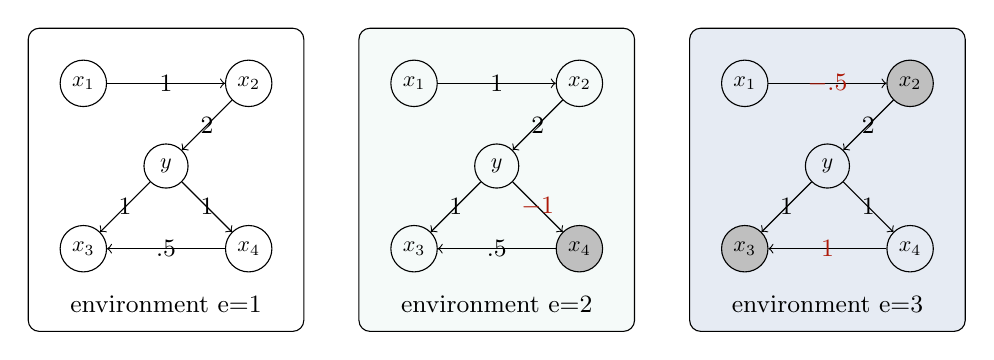
\begin{tikzpicture}[scale=0.7,state/.style={circle, draw, minimum size=0.7cm, scale=0.8}]
    \draw[black, rounded corners] (-1, -4.5) rectangle (4, 1);

    \node[state] at (0,0) (x1) {$x_1$};
    \node[state] at (1.5,-1.5) (y) {$y$};
    \node[state] at (3,0) (x2) {$x_2$};
        \node[state] at (0,-3)  (x3) {$x_3$};
    \node[state] at (3,-3) (x4) {$x_4$};
    
    \draw[->] (x1) -- node{\small $1$} (x2);
    \draw[->] (x2) -- node{\small $2$} (y);
    \draw[->] (y) -- node{\small $1$} (x3);
    \draw[->] (y) -- node{\small $1$} (x4);
    \draw[->] (x4) -- node{\small $.5$} (x3);
    \draw node at (1.5, -4) {\small environment e=1};
    
    \draw[black, fill=mylightblue!10, rounded corners] (5, -4.5) rectangle (10, 1);

    \node[state] at (6,0) (e2x1) {$x_1$};
    \node[state] at (7.5,-1.5) (e2y) {$y$};
    \node[state] at (9,0) (e2x2) {$x_2$};
        \node[state] at (6,-3)  (e2x3) {$x_3$};
    \node[state,fill=gray!50] at (9,-3) (e2x4) {$x_4$};
    
    \draw[->] (e2x1) -- node{\small $1$} (e2x2);
    \draw[->] (e2x2) -- node{\small $2$} (e2y);
    \draw[->] (e2y) -- node{\small $1$} (e2x3);
    \draw[->] (e2y) -- node{\small \myred{$-1$}} (e2x4);
    \draw[->] (e2x4) -- node{\small $.5$} (e2x3);
    \draw node at (7.5, -4) {\small environment e=2};
    
    \draw[black, fill=myblue!10, rounded corners] (11, -4.5) rectangle (16, 1);

    \node[state] at (12,0) (e3x1) {$x_1$};
    \node[state] at (13.5,-1.5) (e3y) {$y$};
    \node[state,fill=gray!50] at (15,0) (e3x2) {$x_2$};
        \node[state,fill=gray!50] at (12,-3)  (e3x3) {$x_3$};
    \node[state] at (15,-3) (e3x4) {$x_4$};
    
    \draw[->] (e3x1) -- node{\small \myred{$-.5$}} (e3x2);
    \draw[->] (e3x2) -- node{\small $2$} (e3y);
    \draw[->] (e3y) -- node{\small $1$} (e3x3);
    \draw[->] (e3y) -- node{\small $1$} (e3x4);
    \draw[->] (e3x4) -- node{\small \myred{$1$}} (e3x3);
    \draw node at (13.5, -4) {\small environment e=3};
\end{tikzpicture}
    \caption{Linear SCMs with different interventions when $p=4$ and $|\mathcal{E}|=3$. Here $z_5=y$, $S^*=\{2\}$, and we omit the dependence on the exogenous variables $u_1,\ldots, u_5$ for a clear presentation. The arrow from node $i$ to node $j$ is marked by $B_{j,i}^{(e)}$ if $B_{j,i}^{(e)} \neq 0$. We can treat $e=1$ as the observational environment and $e=2,3$ as interventional environments. One intervention is performed to the mechanisms of variable $x_4$ (gray shadowed) in environment $e=2$, and simultaneously interventions on variable $x_2$, $x_3$ (gray shadowed) are applied in environment $e=3$. }
    \label{fig:linear-scm-example}
\end{figure}

Consider the following $|\mathcal{E}|$ SCMs on $p+1$ variables $\bz = (x_1,\ldots, x_p, y) \in \mathbb{R}^{p+1}$, that for any $e\in \mathcal{E}$, the following assignments holds
\begin{align}
\label{eq:general-scm-example}
\begin{split}
x^{(e)}_j := z_j^{(e)} &\gets {f^{(e)}_j}(\bz^{(e)}_{{\mathtt{pa}(j)}}, {u_{j}^{(e)}}), ~~~~~~~~~~~~~~~~~~~~ j = 1,\ldots, p\\
y^{(e)} := z_{p+1}^{(e)} &\gets ({\bbeta^*})^\top_{{\mathtt{pa}(p+1)}} \bx^{(e)}_{{\mathtt{pa}(p+1)}} + {u_{p+1}^{(e)}},
\end{split}
\end{align} where all the $\bu^{(e)} = (u_1^{(e)}, \ldots, u_{p+1}^{(e)})$ are independent across different environments and also have independent, zero mean entries. Here the direct cause relationship $\mathtt{pa}: [p+1] \to 2^{[p+1]}$ and the function $f_{p+1}(\bx^{(e)}_{\mathtt{pa}(p+1)}, u_{p+1}^{(e)})=({\bbeta^*})^\top_{{\mathtt{pa}(p+1)}} \bx^{(e)}_{{\mathtt{pa}(p+1)}} + {u_{p+1}^{(e)}}$ are both invariant across different $e\in \mathcal{E}$. The structural assignments $f^{(e)}_j$ for variables $x_j^{(e)}$ and the distribution of exogenous variables $u_j^{(e)}$ may vary among different environments. We use the superscript $(e)$ to emphasize this heterogeneity. We use $\bz$ in the assignments \eqref{eq:general-scm-example} to emphasize that $y$ can be the direct cause of some variables $x_j$. We can see that the heterogeneity may come from performing do-interventions on variables other than $y$ (which will result in different $f_j^{(e)}$ or distribution $u_j^{(e)}$). \cref{fig:linear-scm-example} provides an example of the model \eqref{eq:general-scm-example}.  Here we consider the case where there are no hidden confounders and the system is not anti-causal, since the model misspecification in either direction cannot be addressed without imposing further structural assumptions. 

It is easy to verify that the above model \eqref{eq:general-scm-example} is an instance of the problem formulation discussed in  \cref{subsec:problem-formulation} with the important variable set $S^*=\mathtt{pa}(p+1)$ and the true parameter $\bbeta^*$. Moreover, the set $S^*$ and the parameter $\bbeta^*$ have precise meanings in the context of SCM. Specifically, $S^*$ is the set of \emph{direct causes} of the response variable. From a traditional viewpoint of causal inference, for each $j\in S^*$, the corresponding coefficient $\beta_j^*$ measures how the outcome $y$ will change if we only apply intervention on the variable $x_j$.  

\section{Methodology}
\label{sec:method}

\subsection{Focused Linear Invariance Regularizer}
\label{subsec:focused-regularizer}

As discussed in \cref{prop:necessary-multiple-envs} and \cref{subsec:problem-formulation}, it is necessary to leverage the conditional expectation invariance structure across heterogeneous environments. The straightforward idea is to impose a conditional expectation invariance to the solution $\bar{\bbeta}$ we find. That is, we wish our solution $\bar{\bbeta}$ to satisfy
\begin{align*}
    \forall e\in \mathcal{E}, ~~~~~~ \mathbb{E}\left[y^{(e)} \big |\bx^{(e)}_{\supp(\bar{\bbeta})}\right] \equiv \bar{\bbeta}^\top \bx^{(e)}
\end{align*} from {a population perspective}. To implement the idea efficiently, we consider the variational principle that, for any $e\in \mathcal{E}$ and given $\bbeta \in \mathbb{R}$ with support set $S$, 
\begin{align}
     \mathbb{E}[y^{(e)}|\bx_{S}^{(e)}] = \bbeta^\top_S \bx_S^{(e)} ~~&\Leftrightarrow~~ \mathbb{E} \left[ \left(y^{(e)} - \bbeta^\top_S \bx^{(e)}_S\right) g(\bx_S^{(e)})\right] = 0  ~~~~~~ \forall g ~\text{with}~ \mathbb{E} [ |g(\bx^{(e)}_S)|^2 ] < \infty \nonumber \\
     &\overset{(a)}{\Rightarrow} ~~ \mathbb{E} \left[ \left(y^{(e)} - \bbeta^\top_S \bx^{(e)}_S\right) g(\bx_S^{(e)})\right] = 0  ~~~~~~\forall g~\mathrm{linear} \nonumber\\
     &\Leftrightarrow ~~ \mathbb{E} \left[ \left(y^{(e)} - \bbeta^\top_S \bx^{(e)}_S\right) \bx_j^{(e)}\right] = 0 ~~~~~~~~~~~ \forall j \in S \nonumber \\
     &\Leftrightarrow ~~ \nabla_j \mathsf{R}^{(e)}(\bbeta) = 0 ~~~~~~~~~~~~~~~~~~~~~~~~~~~~~~~ \forall j \in S \label{eq:fr-final-condition}
\end{align} where the statements connected by ``$\Leftrightarrow$'' are equivalent and $\mathsf{R}^{(e)}(\bbeta)$ is defined by \eqref{eq:def-l2-risk}, and we make a relaxation in $(a)$ such that the last statement $\nabla_S \mathsf{R}^{(e)}(\bbeta) = 0$ is a necessary but not sufficient condition for $\mathbb{E}[y^{(e)}|\bx_S^{(e)}] = \bbeta^\top_S\bx_S^{(e)}$. 

Based on the above derivations, we propose to minimize a \emph{focused linear invariance regularizer}, whose population-level form $\mathsf{J}(\bbeta; \bomega)$ can be written as
\begin{align}
\label{eq:invariant-regularizer-population}
\mathsf{J}(\bbeta;\bomega) = \sum_{j=1}^p \mathds{1}\{\beta_j \neq 0\} \sum_{e\in \mathcal{E}} \frac{\omega^{(e)}}{4} |\nabla_j \mathsf{R}^{(e)}(\bbeta)|^2,
\end{align} where $\bomega = (\omega^{(e)})_{e\in \mathcal{E}} \in \mathbb{R}^{|\mathcal{E}|}$ are pre-determined weights associated with environments $\mathcal{E}$ satisfying $\sum_{e\in \mathcal{E}} \omega^{(e)}=1$ and $\omega^{(e)} > 0$ for any $e\in \mathcal{E}$. Some typical choices of $\bomega$ can be $\omega^{(e)} = 1/|\mathcal{E}|$ or $\omega^{(e)} = n^{(e)} / (\sum_{e'\in \mathcal{E}} n^{(e')})$. The word ``\emph{focused}'' emphasizes that we only penalize the gradient in the direction of non-zero coordinates due to the statement \eqref{eq:fr-final-condition}.  See \cite{fan2014endogeneity} for a similar idea for dealing with endogeneity.

We first analyze what it implies when $\mathsf{J}(\bbeta; \bomega)$ attains its global minima. Since $S^*$ is CE-invariant across environments $\mathcal{E}$ according to our assumption, we have $\mathsf{J}(\bbeta^*;\omega)=0$ and this implies the global minima of the loss function $\mathsf{J}(\bbeta;\omega)$ is $0$. Moreover, for a fixed $\tilde{\bbeta}$ with support set $\tilde{S}$, it is easy to see that
\begin{align*}
    \mathsf{J}(\tilde{\bbeta};\bomega) = 0 ~~&\Leftrightarrow~~ \forall e\in \mathcal{E}, ~\nabla_{\tilde{S}} \mathsf{R}^{(e)}(\tilde{\bbeta}) = 0 \\
    ~~&\Leftrightarrow ~~\forall e\in \mathcal{E}, ~\tilde{\bbeta} \in \argmin_{\supp(\bbeta) \subseteq \tilde{S}} \mathsf{R}^{(e)}(\bbeta).
\end{align*}
Therefore, though $\mathsf{J}(\tilde{\bbeta};\omega) = 0$ (attaining its global minima) does not imply that the selected variables set $\tilde{S}$ is \emph{CE-invariant} across environments $\mathcal{E}$, we argue that $\mathsf{J}(\tilde{\bbeta};\bomega) = 0$ indeed indicates that the select variable set $\tilde{S}$ is \emph{LLS-invariant} across environments $\mathcal{E}$, which can be defined as follows.
\begin{definition}[LLS-invariant Set] We say a variable set $S \subseteq [p]$ is \textbf{linear least squares invariant} (LLS-invariant) across environments $\mathcal{E}$ if there exists some $\bbeta$ with support set $S$ such that
\begin{align}
\label{eq:lls-invariant}
    \forall e\in \mathcal{E}, ~~~~~~ \bbeta \in \argmin_{\supp(\bbeta) \subseteq S} \mathbb{E} \left[ |y^{(e)} - \bbeta^\top \bx^{(e)}|^2 \right].
\end{align}
\end{definition}

LLS-invariance is weaker than CE-invariance because the CE-invariance of $S^\star$ implies the LLS-invariance of $S^\star$ while the converse is false.  In this paper, we only leverage linear information to facilitate LLS-invariance on the solution we find. That is what the word ``\emph{linear}'' in our regularizer's name emphasizes. According to the above discussion of the relaxation in $(a)$, we can incorporate more hand-crafted nonlinear features other than linear feature $x_j$ in the \emph{focused invariance regularizer} to somewhat strengthen the degree of invariance. For example, consider the following enhanced regularizer that includes another marginal nonlinear feature $h(\cdot)$ in,
\begin{align}
\label{eq:lls-invariant-nonlinear-feat}
    \mathsf{J}_{h}(\bbeta;\bomega) = \sum_{j=1}^p \mathds{1}\{\beta_j \neq 0\} \sum_{e\in \mathcal{E}} \omega^{(e)} \left\{ \left| \mathbb{E}[ \hat{\varepsilon}^{(e)}_{\bbeta} \bx_j^{(e)}] \right|^2 + \left| \mathbb{E}[ \hat{\varepsilon}^{(e)}_{\bbeta} h(\bx_j^{(e)}) ] \right|^2\right\},
\end{align} where $\hat{\varepsilon}^{(e)}_{\bbeta} = y^{(e)} - \bbeta^\top \bx^{(e)}$. Specifically, we can take $h(u) = u^2$ or $h(u) = \cos(u)$.

Though LLS-invariance is weaker than CE-invariance, these two types of invariance are equivalent under some specific models. For example, suppose $\mu^{(e)}_{\bx, y}$ are all joint Gaussian distribution for any $e\in \mathcal{E}$. In that case, it is easy to verify that if a set $S$ is LLS-invariant, then $S$ is also CE-invariant using the fact that uncorrelatedness implies independence for joint Gaussian random variables. In this case, the enhanced regularizer \eqref{eq:lls-invariant-nonlinear-feat} would have no advantages over the most simple linear one \eqref{eq:invariant-regularizer-population}.


\subsection{Our Approach: EILLS}

Given data $\{\mathcal{D}^{(e)}\}_{e\in \mathcal{E}} = \{\{(\bx_i^{(e)},y_i^{(e)})\}_{i=1}^{n^{(e)}}\}_{e\in \mathcal{E}}$ from heterogeneous environments, the empirical-level \emph{focused linear invariance regularizer} with weights $\bomega$ can be written as
\begin{align}
\label{eq:invariant-regularizer-empirical}
    \hat{\mathsf{J}}(\bbeta;\bomega) = \sum_{j=1}^p \mathds{1}\{\beta_j \neq 0\} \sum_{e\in \mathcal{E}} \omega^{(e)} \left| \hat{\mathbb{E}}[x_j^{(e)} (y^{(e)} - \bbeta^\top \bx^{(e)})]\right|^2.
\end{align} 
Recall that $\hat{\mathsf{R}}^{(e)}(\bbeta)$ defined in \eqref{eq:def-l2-risk} is the empirical $L_2$ loss in environment in $e\in \mathcal{E}$. We also define the following \emph{pooled empirical $L_2$ loss} over all the environments: for $\bbeta \in \mathbb{R}^p$,
\begin{align}
\label{eq:pooled-l2-risk-empirical}
    \hat{\mathsf{R}}(\bbeta;\bomega) = \sum_{e\in \mathcal{E}} \omega^{(e)} \hat{\mathsf{R}}^{(e)}(\bbeta) = \sum_{e\in \mathcal{E}}  \frac{\omega^{(e)}}{n^{(e)}} \sum_{i=1}^{n^{(e)}} \{ y^{(e)}_i - \bbeta^\top \bx^{(e)}_i \}^2.
\end{align}
The \emph{environment invariant linear least squares (EILLS)} estimator $\hat{\bbeta}_{\mathsf{Q}}$ is defined by minimizing the following objective function:
\begin{align}
\label{eq:eills-objective-q}
    \hat{\mathsf{Q}}(\bbeta; \gamma, \bomega) = \hat{\mathsf{R}}(\bbeta;\bomega) + \gamma \hat{\mathsf{J}}(\bbeta;\bomega),
\end{align} which is a linear combination of the pooled empirical $L_2$ loss $\hat{\mathsf{R}}(\bbeta;\bomega)$ and focused linear invariance regularizer $\hat{\mathsf{J}}(\bbeta;\bomega)$ with weights $(1,\gamma)$ for some given hyper-parameter $\gamma \in \mathbb{R}^+$. We also define the population analogs of the EILLS objective function as follows:
\begin{align}
\label{eq:eills-objective-q-population}
    \mathsf{Q}(\bbeta;\gamma,\bomega) = \mathsf{R}(\bbeta; \bomega) + \gamma \mathsf{J}(\bbeta; \bomega) ~~~~ \text{with} ~~~~ \mathsf{R}(\bbeta; \bomega) = \sum_{e\in \mathcal{E}} \omega^{(e)} \mathbb{E} \left[|y^{(e)} - \bx^\top \bx^{(e)}|^2 \right].
\end{align}

The focused regularizer $\mathsf{J}(\bbeta; \bomega)$ can screen out all linear spurious variables when $\gamma$ is large enough.  This can lead to a low-dimensional problem and be sufficient for many applications. However, some linear exogenous variables that do not contribute to explaining $y$ can still survive after the screening. They can be eliminated further by introducing an $\ell_0$ penalty.
This leads us to considering the $\ell_0$ regularized EILLS estimator $\hat{\bbeta}_{\mathsf{L}}$ that minimizes the following objective:
\begin{align}
\label{eq:eills-objective-l}
    \hat{\mathsf{L}}(\bbeta; \lambda, \gamma, \bomega) = \hat{\mathsf{Q}}(\bbeta; \gamma, \bomega) + \lambda \|\bbeta\|_0 =  \hat{\mathsf{R}}(\bbeta;\bomega) +  \gamma \hat{\mathsf{J}}(\bbeta;\bomega)  +  \lambda \|\bbeta\|_0
\end{align} with given hyper-parameter $\lambda$.  This helps reduce variables that are uncorrelated to residuals and $y$.

At the methodology level, our method has a close connection to the FGMM estimator in \cite{fan2014endogeneity} and the invariant risk minimization \citep{arjovsky2019invariant} framework; see detailed connections and differences in \aosversion{Appendix~{\color{blue}D}}{\cref{sec:discussion}}. 

\medskip

\noindent \textbf{Practical Concerns} The current estimator has some combinatorial nature in optimization of \eqref{eq:invariant-regularizer-empirical} and involves an additional hyper-parameter $\gamma$. For the first concern, we show that one can use the Gumbel \citep{jang2016categorical} trick introduced by a follow-up work \cite{gu2024causality} to make variants of gradient descent continue to work in practice; see how to adopt Gumbel approximation to transform \eqref{eq:eills-objective-q} to a continuous optimization program and some simulation studies when $p=70$ in \aosversion{Appendix \blue{D.6}}{\cref{sec:gumbel}}. We also provide some guidance on how to tune the hyper-parameter $\gamma$ in practice; see \aosversion{Appendix \blue{D.7}}{\cref{sec:gamma-tune}}.


\section{Theory}
\label{sec:theory}

 To simplify the presentation, we consider the case of balanced data with equal weights, that is, $n^{(e)} \equiv n$ and $\omega^{(e)} \equiv 1/|\mathcal{E}|$, and defer the results of varying $(n^{(e)}, \omega^{(e)})$ to \aosversion{Appendix~\blue{A}}{\cref{sec:theory:general}}. 
Define the pooled covariance matrix $\bSigma = \frac{1}{|\mathcal{E}|} \sum_{e\in \mathcal{E}} \bSigma^{(e)}$. We first impose some regularity conditions for theoretical analysis.

\begin{condition}
\label{cond0-model-main}
    For each $e\in \mathcal{E}$,  $(\bx_1^{(e)}, y_1^{(e)}), \ldots, (\bx_{n}^{(e)}, y_{n}^{(e)})$ are i.i.d. copies of $(\bx^{(e)}, y^{(e)}) \sim \mu^{(e)}$, where $\mu^{(e)}$ belongs to $\mathcal{U}_{\bbeta^*, \sigma^2}$ for some $\sigma^2$. The data from different environments are also independent.  We set $\omega^{(e)} \equiv 1/|\mathcal{E}|$. 
\end{condition}

\begin{condition}
\label{cond1-well-condition-main}
    There exists some universal constants $\kappa_L \in (0,1]$ and $\kappa_U \in [1,\infty)$ such that
    \begin{align}
        \forall e\in \mathcal{E}, ~~~~~~~~~~ \kappa_L \bI_p \preceq \bSigma^{(e)} \preceq \kappa_U \bI_p.
    \end{align}
\end{condition}

\begin{condition}
\label{cond2-subgaussain-x-main}
    There exists some universal constant $\sigma_x \in [1,\infty)$ such that
    \begin{align}
        \forall e\in \mathcal{E}, \bv \in \mathbb{R}^p, ~~~~~~~~~~  \mathbb{E} \left[\exp\left\{\bv^\top {\bSigma}^{-1/2}\bx^{(e)}\right\}\right]  \le \exp\left(\frac{\sigma_x^2}{2} \cdot \|\bv\|_2^2\right).
    \end{align}
\end{condition}

\begin{condition}
\label{cond3-sub-gaussian-eps-main}
    There exists some universal constant $\sigma_\varepsilon \in \mathbb{R}^+$ such that,
    \begin{align}
        \forall e\in \mathcal{E}, \lambda \in \mathbb{R}, ~~~~~~~~~~ \mathbb{E} [e^{\lambda \varepsilon^{(e)}}] \le e^{\frac{1}{2} \lambda^2 \sigma_\varepsilon^2}.
    \end{align}
\end{condition}

\cref{cond0-model-main} is the basic setup of our multi-environment linear regression described in \cref{subsec:problem-formulation}. \cref{cond1-well-condition-main}--\ref{cond3-sub-gaussian-eps-main} are standard in high-dimensional linear regression analysis. We focus on the centered covariate case that $\mathbb{E}[\bx^{(e)}] = \bm{0}$, and it can be easily generalized to the non-centered counterpart.  The lower bound on the smallest eigenvalue, $\kappa_L$, is to establish non-asymptotic error bounds on $\ell_2$ norm $\|\hat{\bbeta}-\bbeta^*\|_2$. To simplify expressions in our results, we set $\kappa_U \land \sigma_x \ge 1$ and $\kappa_L \le 1$, thus avoiding repeated use of $(\kappa_U \lor 1)$, $(\sigma_x \lor 1)$, and $(\kappa_L^{-1} \lor 1)$. We adopt simple sub-Gaussian conditions to convey our main message. It is possible to relax the above conditions and derive a similar result. For example, one can replace the sub-Gaussian condition of the noise $\varepsilon^{(e)}$ with the sub-Weibull condition \citep{vladimirova2020sub}. One can also substitute the joint sub-Gaussian condition of the covariate with the marginal sub-Weibull condition and show that the EILLS objective \eqref{eq:eills-objective-q} with folded concave penalty function introduced by \cite{fan2001variable} has certain oracle property.

\subsection{Pooled Linear Spurious Variables and the Bias of Pooled Least Squares}
\label{subsec:linear-spurious-variable}

We first define \emph{pooled linear spurious variables} and demonstrate that the vanilla pooled least squares method is an inconsistent estimator in the presence of pooled linear spurious variables.

\begin{definition}[Pooled Linear Spurious Variables] We let $G$ be the index set of all pooled linear spurious variables in environments $\mathcal{E}$ concerning the uniform weights $\omega^{(e)}\equiv 1/|\mathcal{E}|$, that is,
        $G = \{j \in [p]:  \sum_{e\in \mathcal{E}} \mathbb{E}[x_j^{(e)}\varepsilon^{(e)}] \neq 0 \}$. We say $x_j$ is a pooled linear spurious variable if $j\in G$.
\end{definition}


The following proposition characterizes the properties of pooled least squares.

\begin{proposition}[Properties of Pooled Least Squares]
\label{prop:pooled-least-squares-main}
 Assume Conditions \ref{cond0-model-main}--\ref{cond3-sub-gaussian-eps-main} hold. Then, there exists some $\bar{\bbeta}^{\mathsf{R}} \in \mathbb{R}^p$ satisfying $\frac{1}{\kappa_U} \|\frac{1}{|\mathcal{E}|}\sum_{e\in \mathcal{E}} \mathbb{E} [\varepsilon^{(e)} \bx^{(e)}] \|_2 \le \|\bar{\bbeta}^{\mathsf{R}} - \bbeta^*\|_2 \le \frac{1}{\kappa_L} \|\frac{1}{|\mathcal{E}|}\sum_{e\in \mathcal{E}} \mathbb{E} [\varepsilon^{(e)} \bx^{(e)}] \|_2$ 
    such that, for any $\bbeta \in \mathbb{R}^p$,
    \begin{align}
    \label{eq:pooled-least-square-strong-convexity-main}
        \mathsf{R}(\bbeta) - \mathsf{R}(\bar{\bbeta}^{\mathsf{R}}) = \|\bSigma^{1/2}(\bbeta - \bar{\bbeta}^{\mathsf{R}})\|_2^2.
    \end{align} Moreover, there exist universal constants $c_1$ and $c_2$ such that if $n\cdot |\mathcal{E}| \ge c_1 \sigma_x^4(p + t)$, then the pooled least      squares estimator $\hat{\bbeta}_{\mathsf{R}}$ minimizing \eqref{eq:pooled-l2-risk-empirical} satisfies
    \begin{align*}
        \|{\bSigma}^{1/2}(\hat{\bbeta}_{\mathsf{R}} - \bar{\bbeta}^{\mathsf{R}})\|_2 \le c_2 \sigma_x \left(\sigma_\varepsilon + \sigma_x \|{\bSigma}^{1/2}(\bar{\bbeta}^{\mathsf{R}} - \bbeta^*)\|_2\right) \sqrt{\frac{p + t}{{ n\cdot |\mathcal{E}|}}}
    \end{align*} with probability at least $1-2e^{-t}$.
\end{proposition}

From \cref{prop:pooled-least-squares-main}, we observe that $\delta_{\mathtt{b}}=\|\bar{\bbeta}^{\mathsf{R}} - \bbeta^*\|_2$, which can be interpreted as the bias of the pooled least squares, satisfies $\delta_{\mathtt{b}} \asymp \left\||\mathcal{E}|^{-1} \sum_{e\in \mathcal{E}}  \mathbb{E} [\varepsilon^{(e)} \bx^{(e)}] \right\|_2$. \cref{prop:pooled-least-squares-main} thus indicates that, for large enough $n$,
\begin{align*}
    \|\hat{\bbeta}_{\mathsf{R}} - \bbeta^*\|_2 \asymp \left\|\frac{1}{|\mathcal{E}|}\sum_{e\in \mathcal{E}} \mathbb{E}[\varepsilon^{(e)} \bx^{(e)}]\right\|_2.
\end{align*} 
Therefore, the pooled least squares can be a fair estimate of $\bbeta^*$ only when the biases from each environment happen to cancel: $\sum_{e\in \mathcal{E}} \mathbb{E} [\varepsilon^{(e)} x_j^{(e)}] = o(|\mathcal{E}|)$ for any $j\in \mathcal{E}$. Moreover, the strong convexity with respect to $\bar{\bbeta}^{\mathsf{R}}$ \eqref{eq:pooled-least-square-strong-convexity-main} suggests that this issue persists for penalized least squares.



\subsection{Local Strong Convexity for Population Loss}
\label{subsec:strong-convexity}

We first examine the population EILLS loss \eqref{eq:eills-objective-q-population} when $G\neq \emptyset$. Specifically, we show that with a large enough $\gamma$, the population EILLS loss satisfies certain strong convexity with respect to $\bbeta^*$ under the following identification condition. 


\begin{condition}[Identification]
\label{cond-ident-main}
    For any $S\subseteq [p]$ satisfying $S \cap G \neq \emptyset$, there exists some $e, e'\in \mathcal{E}$ such that $\bbeta^{(e, S)} \neq \bbeta^{(e',S)}$, where $\bbeta^{(e,S)}$ is defined in \eqref{eq:local-minimizer}.
\end{condition} 


\begin{remark}[Near Minimal Identification Condition]
It is worth noticing that the above identification condition is minimal if only linear information is considered. To see this, consider the case where $(\bx^{(e)}, y^{(e)})$ are all multivariate normal distributions, a violation of \cref{cond-ident-main} implies that there exist some $\tilde{\bbeta}$ with support set $\tilde{S}$ containing variables outside $S^\star$ such that
\begin{align*}
    \forall e\in \mathcal{E}, ~~~~~ \mathbb{E}[y^{(e)}|\bx_{\tilde{S}}^{(e)}] \equiv (\tilde{\bbeta}_{\tilde{S}})^\top \bx_{\tilde{S}}^{(e)}.
\end{align*} 
In this case, it is impossible to determine which one among $S^*$ and $\tilde{S}$ is the true important variable set because they are all CE-invariant across $\mathcal{E}$ and $\tilde{S}\setminus S^*\neq \emptyset$. 
\end{remark}

\begin{theorem}[Strong Convexity with respect to $\bbeta^*$] 
\label{thm:global-strong-convexity-main}
Assume Conditions \ref{cond0-model-main}--\ref{cond1-well-condition-main} and \ref{cond-ident-main} hold. Then $\bbeta^*$ is the unique minimizer of $\mathsf{Q}(\bbeta;\gamma, \bomega)$ for large enough $\gamma$: for any $\epsilon \in (0, 1)$ and any $\gamma\ge \epsilon^{-1} \gamma^*$ with
\begin{align}
\label{eq:thm1-gamma-star-main}
    \gamma^* = (\kappa_L)^{-3} \sup_{S: S\cap G \neq \emptyset} \left(\mathsf{b}_S/\bar{\mathsf{d}}_S\right),
\end{align} where $\mathsf{b}_S = \|\frac{1}{|\mathcal{E}|}\sum_{e\in \mathcal{E}} \mathbb{E} [\varepsilon^{(e)} \bx_S^{(e)}] \|^2_2$ and $\bar{\mathsf{d}}_S = \sum_{e\in \mathcal{E}} \frac{1}{|\mathcal{E}|} \|\bbeta^{(e,S)} - \bar{\bbeta}^{(S)}\|_2^2$
 with $\bar{\bbeta}^{(S)}=\frac{1}{|\mathcal{E}|} \sum_{e'\in \mathcal{E}} \bbeta^{(e',S)}$, we have
\begin{align}
\label{eq:thm1-jsc-condition-main}
    \mathsf{Q}(\bbeta;\gamma, \bomega) - \mathsf{Q}(\bbeta^*;\gamma, \bomega) \ge (1-\epsilon) \|\bSigma^{1/2}(\bbeta - \bbeta^*)\|_2^2 + \kappa_L^2 (\gamma - \epsilon^{-1}\gamma^*) \bar{\mathsf{d}}_{\supp(\bbeta)}.
\end{align}
\end{theorem}

Note $\bar{\mathsf{d}}_S>0$ for any $S\cap G \neq \emptyset$ under \cref{cond-ident-main}. \cref{thm:global-strong-convexity-main} provides a generic condition under which $\bbeta^*$ is the global optimal of the population-level EILLS objective \eqref{eq:eills-objective-q-population} with a non-asymptotic critical threshold for $\gamma$. Moreover, a detailed characterization of global optimality \eqref{eq:thm1-jsc-condition-main}, which is slightly stronger than strong convexity, is also established.  The strong convexity with respect to the target function $\bbeta^*$ lays the foundation to derive faster convergence rate to $\bbeta^*$ \citep{van1996weak, wainwright2019high}.

\begin{remark}[Interpretation of the Quantities $\mathsf{b}_S$, $\bar{\mathsf{d}}_S$]
Observe that when $S\supseteq S^*$, the bias of the least squares solution in one environment $e\in \mathcal{E}$ is $\bDelta^{(e)} = \bbeta^{(e,S)} - \bbeta^*$. Here we refer to $\mathsf{b}_S$ as bias mean because $\mathsf{b}_S$ is the bias of running least squares on $X_S$ using all the data when $S\supseteq S^*$, that is, $\|\hat{\bbeta}_{\mathsf{R}, S} - \bbeta^*\|_2^2 \asymp \mathsf{b}_S$ by  \cref{prop:pooled-least-squares-main}. At the same time, we have $\bar{\mathsf{d}}_S = \frac{1}{|\mathcal{E}|} \sum_{e\in \mathcal{E}} \|\bDelta^{(e)} - (|\mathcal{E}|^{-1}\sum_{e'\in \mathcal{E}} \bDelta^{(e')})\|_2^2$ provided $S\supseteq S^*$. Thus, the quantity $\bar{\mathsf{d}}_S$ can be interpreted as the variance of bias since it measures the variations of the biases $\bDelta^{(e)}$ among different environments.
\end{remark}

\begin{remark}[Interpretation of the Critical Threshold $\gamma^*$] 
\cref{thm:global-strong-convexity-main} implies that the global optimality of $\bbeta^*$ is guaranteed when $\gamma > \gamma^*$. $\gamma^*$ is the ratio of bias mean to bias variance and will affect both the forthcoming estimation error and variable selection property. As an intuitive example, for the previous cow/camel thought experiment, a reasonable value for $\gamma^*$ is expected when the fractions of cows on grass and camels on sand are both 90\% in $e=0$ and 60\% in $e=1$. Similarly, a moderate $\gamma^*$ is anticipated when fractions are 51\% and 53\%. However, with fractions 90\% and 89\%, $\gamma^*$ is significantly larger, necessitating more data for both accurate estimation and variable selection. 
\end{remark}

\begin{remark}[Interpretation of Small $\gamma$]
In \cref{thm:global-strong-convexity-main}, we show that the invariant parameter $\beta^\star$ will uniquely minimize the EILLS objective when $\gamma$ is larger than some threshold $\gamma^\star$. Yet, it is unclear what is the regularization effect of $\gamma \mathsf{J}$ when $\gamma$ is small. We provide some intuitions on the impact of the regularizer when $\gamma$ is small in \aosversion{Appendix~\blue{D.8}}{\cref{sec:small-gamma}}. 
\end{remark}


We use the toy example below to demonstrate (1) when \cref{cond-ident-main} holds, and (2) how $\gamma^*$ scales in a concrete model, and leave more examples and discussions in \aosversion{Appendix~\blue{A.4}}{\cref{sec:moreex}}.

\begin{example}
\label{ex-h-de}
    Consider the following two-environment linear SCMs with $p=2$:
    \begin{align*}
        x^{(e)}_1 &\gets \sqrt{0.5} \cdot \varepsilon_1 \\
        y^{(e)} &\gets 1\cdot x^{(e)}_1 + \sqrt{0.5} \cdot \varepsilon_0 \\
        x^{(e)}_2 &\gets  {s^{(e)}} \cdot y^{(e)} + \varepsilon_2.  
    \end{align*} Here $\varepsilon_0, \varepsilon_1, \varepsilon_2$ are independent, standard normally distributed exogenous variables. The linear model is $y^{(e)} = (\bbeta^*)^\top \bx^{(e)} + \varepsilon^{(e)}$ with $\bbeta^*=(1,0)$ and $\varepsilon^{(e)} = \sqrt{0.5} \varepsilon_0$. Note that $\mathbb{E}[\varepsilon^{(e)} x_2^{(e)}] = 0.5 s^{(e)}$. When $\omega^{(e)}\equiv 1/2$, the variable $x_2$ will be a pooled linear spurious variable if $s^{(1)}+s^{(2)} \neq 0$. 
    
{\normalfont We focus on the case where the pooled least squares is not consistent, i.e., $s^{(1)} + s^{(2)} \neq 0$. In the well-conditioned regime where $|s^{(1)}| + |s^{(2)}| = O(1)$, by some calculations, we have
    \begin{align*}
        \sqrt{\frac{\mathsf{b}_{\{2\}}}{\bar{\mathsf{d}}_{\{2\}}}} \asymp \frac{|s^{(1)}+s^{(2)}|}{|s^{(2)} - s^{(1)}|} \cdot \frac{1}{|1 - s^{(1)} s^{(2)}|}~~~~~~\text{and}~~~~~~\sqrt{\frac{\mathsf{b}_{\{1,2\}}}{\bar{\mathsf{d}}_{\{1,2\}}}} \asymp \frac{|s^{(1)} + s^{(2)}|}{|s^{(2)} - s^{(1)}|}.
    \end{align*}

First, the \cref{cond-ident-main} holds if $s^{(1)}\neq s^{(2)}$ and $s^{(1)} s^{(2)} \neq 1$. The first inequality is easy to understand, without which the underlying distributions in the two environments are identical. The second inequality is strange at first glance. However, we have $\mathbb{E}[y^{(e)}|x_2^{(e)}] \equiv \frac{s}{s^2+1} x_2^{(e)}$ when $s^{(1)} = s = 1/s^{(2)}$. In this case, it is impossible to identify which of $\{1\}$ and $\{2\}$ are the true important variable set because all the sets are CE-invariant across $\mathcal{E}$. This also demonstrates the necessity of taking the supremum over all sets $S$ with $S\cap G \neq \emptyset$ in \eqref{eq:thm1-gamma-star-main}.

When $s^{(1)} s^{(2)}$ is away from $1$, the critical threshold $\gamma^*$ satisfies $(\gamma^*)^{1/2}\asymp |s^{(1)}+s^{(2)}|/|s^{(2)}-s^{(1)}|$, where the numerator quantifies the strength of spuriousness, and the denominator quantifies the strength of heterogeneity. Hence, a constant-level $\gamma$ can be adopted when the strength of heterogeneity is of the same order as the strength of spuriousness.
}\qed
\end{example}


\subsection{Statistical Analysis of the EILLS Estimator in the Low-dimensional Regime}
\label{subsec:theory-low-dim}

Our statistical analysis of the EILLS estimator focuses on the regime where it is possible to identify $\bbeta^*$, i.e., \cref{cond-ident-main} holds, and when our choice of $\gamma$ satisfies $\gamma \ge 3\gamma^* \lor 1$, where $\gamma^*$ is the quantity defined in  \cref{thm:global-strong-convexity-main}. We let $\gamma \ge 1$ to simplify the presentation. We are now ready to provide a statistical analysis of the EILLS estimator $\hat{\bbeta}_{\mathsf{Q}}$ minimizing \eqref{eq:eills-objective-q}.  The first result is about the sure screening with false positive control.
\begin{theorem}[Non-asymptotic Variable Selection Property]
\label{thm:rate-low-dim-main} Define
\begin{align}
\label{eq:thm2-signal-main}
    \mathsf{s}_+ = \min_{j\in S^*} |\beta_j^*|^2 \qquad \text{and} \qquad \mathsf{s}_- = \min_{S\subseteq [p], S\cap G \neq \emptyset} \bar{\mathsf{d}}_S
\end{align} 
Suppose Conditions \ref{cond0-model-main}--\ref{cond-ident-main} hold, and we choose $\gamma \ge 3\gamma^*\lor 1$ where $\gamma^*$ is defined in  \cref{thm:global-strong-convexity-main}. There exists some universal constants $c_1$--$c_2$ that only depends on $(\kappa_U, \sigma_x, \sigma_\varepsilon)$ such that for any $t>0$, if $n \ge c_1(\gamma/\kappa_L)(p+ \log(|\mathcal{E}|) + t)\{\mathsf{s}_+^{-0.5}+\mathsf{s}_+^{-1}+(\gamma\kappa_L\mathsf{s}_-)^{-0.5}\}$, and $n \cdot |\mathcal{E}| \ge c_2(\gamma/\kappa_L)^2(p+t)\{\mathsf{s}_+^{-1} + (\gamma\kappa_L\mathsf{s}_-)^{-1} + 1\}$, then the EILLS estimator $\hat{\bbeta}_{\mathsf{Q}}$ minimizing \eqref{eq:eills-objective-q} satisfies
\begin{align}
\label{eq:low-dim-variable-selection-main}
    \mathbb{P}\left[S^* \subseteq \supp(\hat{\bbeta}_{\mathsf{Q}}) \subseteq G^c \right] \ge 1-7e^{-t}.
\end{align}
\end{theorem}


Equation \eqref{eq:low-dim-variable-selection-main} reveals that all endogenous variables are screened out when $\gamma$ is sufficiently large. When the choice of $\gamma$ and the curvature $\kappa_L$ are both of constant order, \cref{thm:rate-low-dim-main} implies that with high probability, the EILLS estimator $\hat{\bbeta}_{\mathsf{Q}}$ can eliminate all the pooled linear spurious variables while keeping all the important variables, i.e., \eqref{eq:low-dim-variable-selection-main} holds, if 
\begin{align}
\label{eq:low-dim-n-m-condition-main}
    \frac{n}{p + \log(|\mathcal{E}|)} \gg \mathsf{s}_+^{-1} + \mathsf{s}_{-}^{-1/2} \left(1\lor \frac{\mathsf{s}_{-}^{-1/2}}{|\mathcal{E}|}\right).
\end{align}  Here, the quantities $\mathsf{s}_+$ and $\mathsf{s}_-$ defined in \eqref{eq:thm2-signal-main} can be interpreted as the signal of true important variables and the signal of heterogeneity, respectively. One can expect more data to differentiate whether it is a signal or noise when one of $\mathsf{s}_-$ and $\mathsf{s}_+$ is small. 



When the variable selection property \eqref{eq:low-dim-variable-selection-main} is satisfied, $\hat{S}$ does not contain any pooled linear spurious variables while maintaining all the important variables. In this case, one can provide a good estimate of $\bbeta^*$ by running another least squares constrained on $\hat{S} = \supp(\hat{\bbeta}_{\mathsf{Q}})$ without regularization. In this case, there is no bias anymore. It then follows from \cref{prop:pooled-least-squares-main} that, with high probability, we have the $\ell_2$-error $\{|G^c|/(n \cdot |\mathcal{E}|)\}^{1/2}$ given $\hat{S}\subseteq G^c$. 

When some weak spurious variables exist such that the corresponding absolute value of $\bar{\mathsf{d}}_S$ is small, the EILLS estimator requires a large $n$ to eliminate all these spurious variables. To see this, suppose there exists a weak spurious variable $x_j$ such that $|\mathbb{E}[x_j^{(e)}\varepsilon^{(e)}]| \le \epsilon$ for all the $e\in \mathcal{E}$. Consider the set $\tilde{S} = S^* \cup \{j\}$, it is easy to verify that $\mathsf{b}_{\tilde{S}} \le \varepsilon^2$ and $\bar{\mathsf{d}}_{\tilde{S}} \le \varepsilon^2$. In this case, we require $n\gg n_{*,\mathtt{sel}} \asymp p\epsilon^{-1}( \epsilon^{-1}/\mathcal{|E|} + 1)$ to eliminate variable $x_j$ by \eqref{eq:low-dim-n-m-condition-main}. The next theorem claims that a small $\ell_2$ estimation error $\|\hat{\bbeta}_{\mathsf{Q}} - \bbeta^*\|_2$ can be obtained in the regime where $p \ll n \ll n_{*,\mathtt{sel}}$ regardless of whether EILLS selects the correct variable.

\begin{theorem}[Non-asymptotic $\ell_2$ Error Bound] 
\label{thm:rate-faster-low-dim-main}
Assume Conditions \ref{cond0-model-main}--\ref{cond-ident-main} hold, and we choose $\gamma \ge 3\gamma^*\lor 1$ where $\gamma^*$ is defined in \cref{thm:global-strong-convexity-main}. There exists some universal constants $c_1$--$c_4$ that only depend on $(\kappa_U, \sigma_x)$ such that for any $t>0$, if $n \ge p + \log(2|\mathcal{E}|) + t$ and $n \cdot |\mathcal{E}| \ge c_1 (\gamma/\kappa_L)(p + t)$, then $\hat{\bbeta}_{\mathsf{Q}}$ minimizing \eqref{eq:eills-objective-q} satisfies
\begin{align}
\label{eq:low-dim-rate2}
    \frac{\|\hat{\bbeta}_{\mathsf{Q}} - \bbeta^*\|_2}{\sigma_\varepsilon (\gamma/\kappa_L)}  &\le c_2 \left(\sqrt{\frac{p+t}{n \cdot |\mathcal{E}|}} + \frac{p+\log(|\mathcal{E}|)+t}{n}\right) + c_3 \frac{\sqrt{|S^*|}}{n} \cdot \frac{\log(|\mathcal{E}||S^*|)+t}{\min_{j\in S^*}|\beta^*_j|}
\end{align} with probability at least $1-7e^{-t}$. Moreover, when the additional conditions in \cref{thm:rate-low-dim-main} hold, then
\begin{align}
\label{eq:low-dim-rate1}
    \frac{\|\hat{\bbeta}_{\mathsf{Q}} - \bbeta^*\|_2}{\sigma_\varepsilon (\gamma/\kappa_L)}  &\le c_2 \left(\sqrt{\frac{|{G}^c|+t}{n \cdot |\mathcal{E}|}} + \frac{|{G}^c|+\log(|\mathcal{E}|)+t}{n}\right)
\end{align} occurs with probability at least $1-14e^{-t}$.
\end{theorem} 


In the well-conditioned regime where $\min_{j\in S^*} |\beta_j^*| \gtrsim p^{-1/2}$, $\kappa_L\gtrsim 1$, and $\gamma^*\asymp 1$, one can adopt a constant-level hyper-parameter $\gamma$ such that
\begin{align*}
    \|\hat{\bbeta}_{\mathsf{Q}} - \bbeta^*\|_2 \lesssim \sqrt{\frac{p}{n\cdot |\mathcal{E}|}} + \frac{p}{n}
\end{align*} with high probability provided $n \gtrsim p$. When the first term dominates ($|\mathcal{E}|$ is not too big), the EILLS estimator achieves an optimal linear regression rate. This implies that the EILLS estimator can estimate $\bbeta^*$ well in $\ell_2$ error when there are some weak spurious variables and the number of data points is not large enough to eliminate all the variables in $G$. 

One technical novelty behind Theorems \ref{thm:rate-low-dim-main}--\ref{thm:rate-faster-low-dim-main} and \cref{thm:high-dim-main} later is to apply the localization argument in the analysis of the invariance regularizer to get a faster rate. To see this, we have $\|\hat{\bbeta}_{\mathsf{Q}} - \bbeta^*\|_2^2 \asymp \delta_{n,\mathsf{Q}}^2 \asymp (n\cdot |\mathcal{E}|)^{-1} + n^{-2}$ when $p=O(1)$. The first term is faster than $(n\cdot |\mathcal{E}|)^{-1/2}$ which directly applies uniform concentration, and the second term is faster than $n^{-1} \asymp \sup_{\|\bbeta\|_2 \le 1} |\mathsf{J}(\bbeta) - \mathbb{E}[\hat{\mathsf{J}}(\bbeta)]|$, the (uniform) bias of the invariance regularizer. We use \aosversion{Lemma~\blue{C.4}}{\cref{lemma:instance-dependent-bound-j-lowdim}}, a novel one-side instance-dependent error bound for $\mathsf{J}(\bbeta) - \hat{\mathsf{J}}(\bbeta) + \hat{\mathsf{J}}(\bbeta^*) - \mathsf{J}(\bbeta^*)$ to obtain such a faster rate; see \aosversion{Appendix~\blue{C.3}}{\cref{sec:proof-thm2}}. 

\subsection{Variable Selection Consistency in the High-dimensional Regime}
\label{subsec:theory-high-dim}

 In the high-dimensional regime, we further define $s^* = |S^*|$, $\beta_{\min} = \min_{j\in S^*} |\beta_j^*|$. We need a condition asserting that the sample size $n$ should be large enough for the given hyper-parameter $\gamma$.

\begin{condition}
\label{cond6-n-req-main}
    Suppose that $\log(|\mathcal{E}|)\le C\log p$ and that 
    
\noindent (1) $n \ge c_1 (\gamma/\kappa_L) \left\{(s^* +  \beta_{\min}^{-2})\log p + (\kappa_L\beta_{\min})^{-1} \sqrt{(s^* + \log p) s^*\log p}\right\}$
    
\noindent (2) $n \cdot |\mathcal{E}| \ge c_2 (\gamma/\kappa_L)^2 (s^* \log p ) \{1 + 1/ (\kappa_L \beta_{\min}^2 ) \}$, 
    
\noindent Here $c_1$--$c_2$ are positive universal constants that depend only on $(C,\sigma_x,\kappa_U, \sigma_\varepsilon)$.
\end{condition} 

\begin{theorem}[Variable Selection Consistency in High Dimensions]  
\label{thm:high-dim-main}  Assume Conditions \ref{cond0-model-main}--\ref{cond6-n-req-main} hold, and we choose $\gamma \ge 3\gamma^* \lor 1$ where $\gamma^*$ is defined in \cref{thm:global-strong-convexity-main}. Suppose further that the choice of $\lambda$ satisfies
\begin{align*}
    c_1 \left\{ (\gamma/\kappa_L)^2 \frac{s^*\log p}{n \cdot |\mathcal{E}|} + \epsilon(n) \right\} \le \lambda \le c_2 \kappa_L \beta_{\min}^2,
\end{align*} where $\epsilon(n) = (\gamma/\kappa_L)^2 s^\star (\log p)(s^* + \log p) / n^2 + (\gamma/\kappa_L) \log p \sqrt{n^{-3}(s^* + \log p)}$, and  $c_1, c_2$ are some universal positive constants only depends on $(C,\kappa_U, \sigma_x,\sigma_\varepsilon)$. Then the $\ell_0$ regularized EILLS estimator $\hat{\bbeta}_{\mathsf{L}}$ minimizing \eqref{eq:eills-objective-l} satisfies $\mathbb{P}[\supp(\hat{\bbeta}_{\mathsf{L}}) = S^*] \ge 1-p^{-10}$.
\end{theorem}

We can see that $\epsilon(n)$ is negligible when $|\mathcal{E}| \asymp 1$ and $s^*+\log p = o(n)$ because 
\begin{align*}
    \epsilon(n) \Big/ \left\{ (\gamma/\kappa_L)^2\frac{s^* \log p}{n \cdot |\mathcal{E}|}\right\} \lesssim |\mathcal{E}| \left\{ \frac{s^*+\log p}{n} + 
    \left(\sqrt{\frac{\log p}{n}}\right) \right\} = o(1).
\end{align*} Therefore, in the regime where $\gamma, \kappa_L, |\mathcal{E}|$ are fixed while $n, p, s^*$ may grow, the variable selection consistency can be achieved when 
\begin{align*}
\frac{s^* \log p}{n}\ll \lambda \ll \beta_{\min}^2.
\end{align*}  Recall that for standard $\ell_0$ regularized least squares with sample size $n$, the variable selection consistency can be obtained when $n \gg (s^* + \beta_{\min}^{-2})\log p$ and $\lambda$ satisfies $n^{-1} \log p \ll \lambda \ll \beta_{\min}^2$ \citep{zhang2012general}. Compared to the standard $\ell_0$ regularized least squares, the EILLS estimator needs $n \gg s^* \beta_{\min}^{-2} \log p$ in the fixed number of environments setting.


Another question is how much can the $\ell_0$ regularized EILLS estimator benefit from growing $|\mathcal{E}|$? When $\gamma \asymp\kappa_L \asymp s^*\asymp 1$, \cref{thm:high-dim-main} implies that though achieving variable selection consistency still needs $(1+\beta_{\min}^{-2})\log p = o(n)$ due to \cref{cond6-n-req-main} (1), we can choose a wider range of $\lambda$. To be specific, in this case, the variable selection consistency can be achieved when $\lambda$ satisfies
\begin{align*}
    \left\{\frac{1}{|\mathcal{E}|} + \left(\frac{\log p}{n}\right)^{1/2} \right\} \frac{\log p}{n} \ll \lambda \ll \beta_{\min}^2.
\end{align*} Hence we can choose any $(n\cdot |\mathcal{E}|)^{-1} \log p \ll \lambda \ll \beta_{\min}^2$ in the regime $(\log p) |\mathcal{E}|^2 = o(n)$. This is the same with running $\ell_0$ regularized least squares on total $n\cdot |\mathcal{E}|$ data when $\mathbb{E}[\varepsilon|\bx]\equiv 0$.

With the variable selection consistency given in \cref{thm:high-dim-main}, we can then attain the optimal $\ell_2$-rate by running the least squares on $\supp(\hat{\bbeta}_{\mathsf{L}})$, as if assisted by an oracle.


\section{An Illustration by Structural Causal Model}
\label{sec:simulation}

\begin{figure}[!t]
\centering
\begin{tabular}{cc}
\subfigure[]{
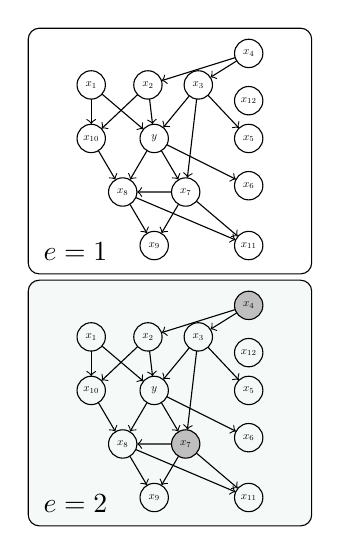
\begin{tikzpicture}[scale=0.4, state/.style={circle, draw, minimum size=0.9cm, scale=0.4}]

\draw[black, rounded corners] (-2, -6) rectangle (7, 1.8);
\draw node at (-0.5, -5.3) {$e=1$};
\node[state] at (0, 0) (x1) {$x_1$};
\node[state] at (2, -1.7) (y) {$y$};
\node[state] at (1.8, 0) (x2) {$x_2$};
\node[state] at (3.4, 0) (x3) {$x_3$};
\node[state] at (5, 1) (x4) {$x_4$}; 
\node[state] at (5, -1.7) (x5) {$x_5$};
\node[state] at (5, -3.2) (x6) {$x_6$};
\node[state] at (3, -3.4) (x7) {$x_7$};
\node[state] at (1, -3.4) (x8) {$x_8$};
\node[state] at (0, -1.7) (x10) {$x_{10}$};
\node[state] at (2, -5.1) (x9) {$x_{9}$};
\node[state] at (5, -5.1) (x11) {$x_{11}$};
\node[state] at (5, -0.5) (x12) {$x_{12}$};

\draw[->] (x1) -- (y);
\draw[->] (x2) -- (y);
\draw[->] (x3) -- (y);
\draw[->] (x1) -- (x10);
\draw[->] (x2) -- (x10);
\draw[->] (x3) -- (x5);
\draw[->] (x4) -- (x2);
\draw[->] (x4) -- (x3);
\draw[->] (y) -- (x6);
\draw[->] (y) -- (x7);
\draw[->] (y) -- (x8);
\draw[->] (x7) -- (x8);
\draw[->] (x10) -- (x8);
\draw[->] (x7) -- (x9);
\draw[->] (x8) -- (x9);
\draw[->] (x7) -- (x11);
\draw[->] (x8) -- (x11);
\draw[->] (x3) -- (x7);

\draw[black, rounded corners, fill=mylightblue!10] (-2, -14) rectangle (7, -6.2);
\draw node at (-0.5, -13.3) {$e=2$};
\node[state] at (0, -8) (e2x1) {$x_1$};
\node[state] at (2, -9.7) (e2y) {$y$};
\node[state] at (1.8, -8) (e2x2) {$x_2$};
\node[state] at (3.4, -8) (e2x3) {$x_3$};
\node[state, fill=gray!50] at (5, -7) (e2x4) {$x_4$}; 
\node[state] at (5, -9.7) (e2x5) {$x_5$};
\node[state] at (5, -11.2) (e2x6) {$x_6$};
\node[state, fill=gray!50] at (3, -11.4) (e2x7) {$x_7$};
\node[state] at (1, -11.4) (e2x8) {$x_8$};
\node[state] at (0, -9.7) (e2x10) {$x_{10}$};
\node[state] at (2, -13.1) (e2x9) {$x_{9}$};
\node[state] at (5, -13.1) (e2x11) {$x_{11}$};
\node[state] at (5, -8.5) (e2x12) {$x_{12}$};

\draw[->] (e2x1) -- (e2y);
\draw[->] (e2x2) -- (e2y);
\draw[->] (e2x3) -- (e2y);
\draw[->] (e2x1) -- (e2x10);
\draw[->] (e2x2) -- (e2x10);
\draw[->] (e2x3) -- (e2x5);
\draw[->] (e2x4) -- (e2x2);
\draw[->] (e2x4) -- (e2x3);
\draw[->] (e2y) -- (e2x6);
\draw[->] (e2y) -- (e2x7);
\draw[->] (e2y) -- (e2x8);
\draw[->] (e2x7) -- (e2x8);
\draw[->] (e2x10) -- (e2x8);
\draw[->] (e2x7) -- (e2x9);
\draw[->] (e2x8) -- (e2x9);
\draw[->] (e2x7) -- (e2x11);
\draw[->] (e2x8) -- (e2x11);
\draw[->] (e2x3) -- (e2x7);

\end{tikzpicture}   
} & 
\subfigure[]{
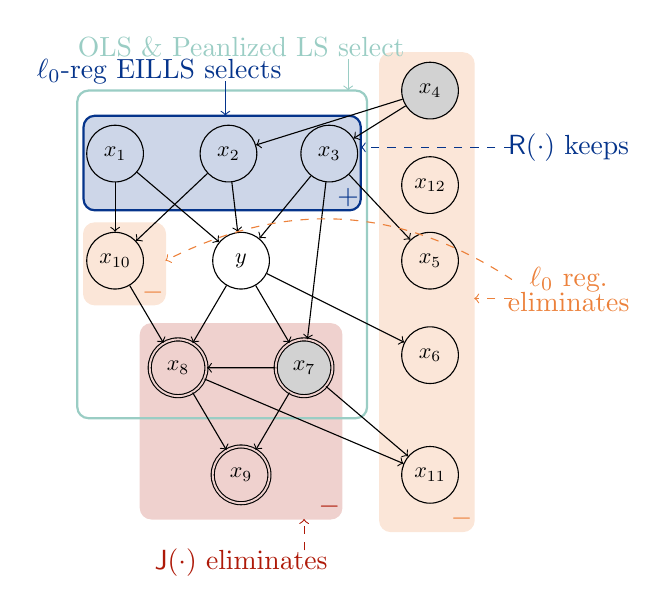
\begin{tikzpicture}[scale=0.8, state/.style={circle, draw, minimum size=0.9cm, scale=0.8}]

\draw[myorange!20, fill=myorange!20, rounded corners] (4.2, -6) rectangle (5.7, 1.6);
\draw[myorange!20, fill=myorange!20, rounded corners] (-0.5, -2.4) rectangle (0.8, -1.1);
\draw[myred!20, fill=myred!20, rounded corners] (0.4, -5.8) rectangle (3.6, -2.7);
\draw[myblue, thick, fill=myblue!20, rounded corners] (-0.5, -0.9) rectangle (3.9, 0.6);
\draw[mylightblue, thick, rounded corners] (-0.6, -4.2) rectangle (4, 1);

\node[state] at (0, 0) (x1) {$x_1$};
\node[state] at (2, -1.7) (y) {$y$};
\node[state] at (1.8, 0) (x2) {$x_2$};
\node[state] at (3.4, 0) (x3) {$x_3$};
\node[state, fill=gray!35] at (5, 1) (x4) {$x_4$}; 
\node[state] at (5, -1.7) (x5) {$x_5$};
\node[state] at (5, -3.2) (x6) {$x_6$};
\node[state, double=myred!20, double distance=0.7pt, fill=gray!35] at (3, -3.4) (x7) {$x_7$};
\node[state, double=myred!20, double distance=0.7pt] at (1, -3.4) (x8) {$x_8$};
\node[state] at (0, -1.7) (x10) {$x_{10}$};
\node[state, double=myred!20, double distance=0.7pt] at (2, -5.1) (x9) {$x_{9}$};
\node[state] at (5, -5.1) (x11) {$x_{11}$};
\node[state] at (5, -0.5) (x12) {$x_{12}$};

\draw[myblue] node at (3.7, -0.7) {$+$};
\draw[myorange] node at (5.5, -5.8) {$-$};
\draw[myorange] node at (0.6, -2.2) {$-$};
\draw[myred] node at (3.4, -5.6) {$-$};

\draw[->] (x1) -- (y);
\draw[->] (x2) -- (y);
\draw[->] (x3) -- (y);
\draw[->] (x1) -- (x10);
\draw[->] (x2) -- (x10);
\draw[->] (x3) -- (x5);
\draw[->] (x4) -- (x2);
\draw[->] (x4) -- (x3);
\draw[->] (y) -- (x6);
\draw[->] (y) -- (x7);
\draw[->] (y) -- (x8);
\draw[->] (x7) -- (x8);
\draw[->] (x10) -- (x8);
\draw[->] (x7) -- (x9);
\draw[->] (x8) -- (x9);
\draw[->] (x7) -- (x11);
\draw[->] (x8) -- (x11);
\draw[->] (x3) -- (x7);

\draw[mylightblue] (2, 1.7) node{OLS \& Peanlized LS select};
\draw[->, mylightblue] (3.7, 1.5) -- (3.7, 1);

\draw[myblue] (0.7, 1.3) node{$\ell_0$-reg EILLS selects};
\draw[->, myblue] (1.75, 1.15) -- (1.75, 0.6);

\draw[myred] (2, -6.5) node{$\mathsf{J}(\cdot)$ eliminates};
\draw[->, dashed, myred] (3, -6.3) to (3, -5.8);

\draw[myorange] (7.2, -2) node{$\ell_0$ reg.};
\draw[myorange] (7.2, -2.35) node{eliminates};
\draw[->, dashed, myorange] (6.3,-2.3) to (5.7, -2.3);
\draw[->, dashed, myorange] (6.3,-2) to[bend right] (0.8, -1.7);

\draw[myblue] (7.2, 0.1) node{$\mathsf{R}(\cdot)$ keeps};
\draw[->, dashed, myblue] (6.3, 0.1) to (3.9, 0.1);

\end{tikzpicture}

}
\end{tabular}


\caption{(a) An illustration of the two-environment model, the SCMs in the two environments share the same induced graph, which is also plotted in (b). The arrow from node $x$ to node $z$ indicates that $x$ is the direct cause of $z$. (b) An illustration of how EILLS works under the two-environment model. The double-circled nodes represent the pooled linear spurious variables.}
\label{fig:scm-variable-selection}
\end{figure}

In this section, we use an example of a structural causal model (with potential interventions on covariates $\bx$) to illustrate how different components of our proposed EILLS objective \eqref{eq:eills-objective-q} and $\ell_0$ regularized EILLS objective \eqref{eq:eills-objective-l} contribute to either seizing the important variables $S^*$ or eliminating pooled linear spurious variables and unrelated variables. Simulations further support intuitive claims\footnote{Scripts to reproduce the simulation result in this section can be found in the supplemental material, see also \href{https://github.com/wmyw96/EILLS}{https://github.com/wmyw96/EILLS}.}.



\noindent \textbf{Model.} Consider a two-environment model ($|\mathcal{E}|=2$). The mechanism of $(\bx, y)$ in each environment is characterized by an SCM. As shown in \cref{fig:scm-variable-selection} (a), the two SCMs share the same direct cause relationship and most of the structural assignments, except that the mechanisms of $x_4$ and $x_7$ are different (gray shadowed); see the detailed structural assignments in \aosversion{Appendix~\blue{D.4}}{\cref{subsec:implementation}}. In this case, the set of important variables $S^*$ is $\{1,2,3\}$, corresponding to the set of direct causes of $y$. The true parameter is $\bbeta^*=(3,2,-0.5,0,\ldots, 0)^\top$. The set of pooled linear spurious variables $G$ is the subset of $y$'s offspring. In this example, $G=\{7,8,9\}$ (denote as double circled node in \cref{fig:scm-variable-selection} (b)).

\noindent \textbf{How EILLS rescues.} First, although vanilla pooled least squares, which minimizing \eqref{eq:pooled-l2-risk-empirical}, can asymptotically eliminate some uncorrelated variables (for example, $\hat{\beta}_{\mathsf{R},12} = o_{\mathbb{P}}(1)$), it will asymptotically select some of the pooled linear spurious variables in $G$ together with other variables related to these variables (for example, some of their ancestors and offsprings) according to \eqref{eq:intro-lse-sol}. For example, it may asymptotically select variables $S_{\mathsf{R}} = \{1, 2, 3, 7, 8, 10\}$ as shown in the \fcolorbox{mylightblue}{white}{\mylightblue{light blue rectangle}}. That is, $|\hat{\beta}_{\mathsf{R},j} - \beta_j| = o_{\mathbb{P}}(1)$ with some $\beta_j\neq 0$ will hold for any $j \in S_{\mathsf{R}}$.

As for our EILLS estimator that minimizes \eqref{eq:eills-objective-q}, if the inclusion of pooled linear spurious variables leads to a shift of best linear predictor (\cref{cond-ident-main}), then, with a large enough $\gamma$, our regularizer \myred{$\hat{\mathsf{J}}$} will eliminate all pooled linear spurious variables in \colorbox{myred!20}{red shadows} for large enough sample size. We add a red ``\myred{$-$}'' in the red shadow to emphasize the regularizer \myred{$\hat{\mathsf{J}}$}'s role in eliminating those pooled linear spurious variables. 
Moreover, including the pooled $L_2$ risk \myblue{$\hat{\mathsf{R}}_{\mathcal{E}}$} will prevent our EILLS objective from collapsing to conservative solutions. Thus it will select all the important variables in \colorbox{myblue!20}{blue shadows}, in which we also use a blue ``\myblue{$+$}'' to underline the pooled $L_2$ risk \myblue{$\hat{\mathsf{R}}_{\mathcal{E}}$}'s impact on keeping all the important variables. 
Finally, the objective \eqref{eq:eills-objective-q} can only guarantee that $\hat{\beta}_{\mathsf{Q},j} = o_{\mathbb{P}}(1)$ for unrelated variables $j$ in \colorbox{myorange!20}{orange shadows}, the inclusion of \myorange{$\ell_0$ regularization} completes the last step towards the target of variable selection consistency: with a properly chosen hyper-parameter $\lambda$, we can eliminate (\myorange{$-$}) these unrelated variables through the \myorange{$\ell_0$ penalty} and only keep the important variables in \fcolorbox{myblue}{white}{\myblue{blue rectangle}}.

\begin{figure}
\centering
\begin{tabular}{ccc}
\subfigure[]{
\includegraphics[scale=0.36]{figures/reg_path.pdf}
}&
\subfigure[]{
\includegraphics[scale=0.36]{figures/l2error_n.pdf}
} &
\subfigure[]{
\includegraphics[scale=0.36]{figures/varsel_n.pdf}
} 
\end{tabular}
\caption{The simulation results for the model in \cref{fig:scm-variable-selection} (a). (a) depicts how the estimated coefficients for the EILLS estimator vary across hyper-parameter $\gamma$ in one trial when $n=300$: we use \myblue{blue} and \myred{red} solid lines to represent the corresponding coefficients for variables in \myblue{$S^*$} and \myred{$G$}, respectively; and use \myorange{orange} dashed lines to represent the coefficients for other variables. The two gray vertical lines are $\gamma=15$ and $\gamma=3\times 10^3$, respectively. (b) depicts how the average $\ell_2$ errors (based on $500$ replications, shown in log scale) for different estimators (marked with different shapes) change when $n$ grows: `LS $S$' is the estimator that runs least squares on $\bx_S$ using all the data and `PLS' is referred to `LS $[p]$'. 
(c) depicts the average number of selected variables in $S^*$ (\myblue{$+$}) and $G$ (\myred{$\times$}) for the EILLS estimator over $500$ replications.
}
\label{fig:numerical}
\end{figure}

\noindent \textbf{Experimental Justification.} We support the above intuition via simulations, in which the balanced data setting ($n^{(e)} \equiv n$, $\omega^{(e)}\equiv 1/2$) is adopted. Detailed implementation and experimental configurations are presented in \aosversion{Appendix~\blue{D.4}}{\cref{subsec:implementation}}.

Let us first see how EILLS works in practice by visualizing how the estimates of coefficients change over $\gamma \in [0, 10^4]$ in one trial. As shown in \cref{fig:numerical} (a), the pooled least squares running least squares on all the data ($\gamma=0$) will lead to a biased solution, which significantly selects variables in $S_{\mathsf{R}}$. Meanwhile, the EILLS estimator with proper regularization parameter $\gamma \in [15, 3\times 10^3]$ selects variables $\{1,2,3,5\}$: it screens out all the variables in $G$ and keeps all the important variables in $S^*$. \cref{fig:numerical} (a) also demonstrates the necessity of incorporating $L_2$ risk: with a very large $\gamma$ ($\gamma \ge 4\times 10^3$) that the $L_2$ risk is relatively negligible compared with the invariance regularizer, the best (empirical) linear predictor on $\{1,2,3\}$ is not preferred than that on $\{1\}$ by the invariance regularizer.

\cref{fig:numerical} (b) and \cref{fig:numerical} (c) further support the above claims using the average performances over $500$ replications, in which we use fixed $\gamma=20$ for EILLS. As presented in \cref{fig:numerical} (b), the average square of $\ell_2$ estimation error $\|\hat{\bbeta} - \bbeta^*\|_2^2$ for pooled least squares estimator (\mylightblue{$\times$} PLS) does not decrease (remains to be $\approx 4$) as $n$ increases, indicating that it converges to a biased solution. At the same time, the average $\|\hat{\bbeta} - \bbeta^*\|_2^2$ for the EILLS estimator (\myblue{$\blacklozenge$}) decays as $n$ grows (is $\approx 0.1$ when $n=200$) and lies in between that for least squares on $\bx_{G^c}$ (\myorange{$\blacktriangledown$}) and least squares on $\bx_{S^*}$ (\myred{$\blacktriangle$}) when $n\ge 700$. This is expected to happen since the EILLS estimator can not screen out all the uncorrelated variables.  We also report the $\ell_2$ estimation error for the refitted EILLS estimator, which runs OLS on the variable set $\hat{S}$ EILLS selects. It is interesting to see that its performance is slightly worse than the vanilla EILLS estimator; we provide a quantitative explanation in \aosversion{Appendix~\blue{D.5}}{\cref{sec:diagnosis}}.

The variable selection property for EILLS is further demonstrated in \cref{fig:numerical} (c), where the average number of selected variables in $S^*$ (\myblue{$+$}) and $G$ (\myred{$\times$}) is plotted across different $n$. The ``\myblue{$+$}'' curve keeps increasing and is almost $3$ while the ``\myred{$\times$}'' curve decays and approaches $0$, implying that the EILLS will select almost all the variables in $S^*$ and screen out all the variables in $G$ when $n$ grows.

\noindent \textbf{Comparison with Other Invariance Approaches.} In addition, we compare our EILLS approach with other invariance approaches, including invariance causal prediction (ICP) \citep{peters2016causal}, anchor regression (Anchor) \citep{rothenhausler2021anchor}, and invariant risk minimization (IRM) \citep{arjovsky2019invariant}, using the data generating process above. The pooled least squares (PLS) method is also included for comparative purposes. We use EILLS with hyper-parameter $\gamma=20$. For other invariance approaches, the invariance hyper-parameters are chosen in an oracle manner -- we enumerate all the possible hyper-parameters and pick the one that minimizes the $\ell_2$ prediction error $\|\bar{\bSigma}^{1/2}(\hat{\bbeta} - \bbeta^*)\|_2^2$. The implementation details can be found in the Supplemental Material.

The results are shown in \cref{fig:comp} (a). It is apparent that among all the estimators evaluated, the EILLS estimator stands out as the only one capable of consistent estimation. We also provide graphical visualizations of the solutions found by different methods for $n=100$ and $n=1000$ in \cref{fig:comp} (b) and (c), respectively. In these plots, each point $(x, y)$ with marker $m$ represents a solution $\hat{\bbeta}$ that the method $m$ produces. Here, $x$ denotes the relative $\ell_2$ norm restricted to the true important variables set $S^*$, calculated as $\|\hat{\bbeta}_{S^*}\|_2/\|{\bbeta}^*_{S^*}\|_2$; and $y$ represents the relative $\ell_2$ norm restricted to the pooled linear spurious variables set $G$, expressed as $\|\hat{\bbeta}_{G}\|_2/\|\bar{\bbeta}_{G}\|_2$ with $\bar{\bbeta} = \bar{\bbeta}^{([12])}$. 

As depicted in \cref{fig:comp} (b) and (c), the ICP method demonstrates a very conservative nature, failing to select variables in $S^*$ even when $n=1000$. This reveals its lack of guarantees in power even when the sample size is large enough. For other optimization-based methods, the solutions obtained by anchor regression are similar to those found by the pooled least squares. Although the IRM method showcases a slight divergence from PLS, with a tendency to push solutions toward the direction of ``invariance'', this effect remains marginal. In contrast, our EILLS method not only converges to the true parameter $\bbeta^*$ when $n$ is large but also demonstrates commendable performance when the sample size is moderately large ($n=100$).

\begin{figure}
\centering
\begin{tabular}{ccc}
\subfigure[]{
\includegraphics[scale=0.33]{figures/various_method.pdf}
}&
\subfigure[]{
\includegraphics[scale=0.33]{figures/solution-n100.pdf}
} &
\subfigure[]{
\includegraphics[scale=0.33]{figures/solution-n1000.pdf}
} 
\end{tabular}
\caption{The simulation results for different methods using the data generated from the model in \cref{fig:scm-variable-selection} (a). (a) depicts how the average $\ell_2$ prediction errors $\|\bar{\bSigma}^{1/2}(\hat{\bbeta} - \bbeta^*)\|_2^2$ (based on $300$ replications) for different invariance methods (marked with different shapes and colors) changes when $n$ grows. (b) and (c) visualizes the solutions of different methods in 60 replications when $n=100$ and $n=1000$, respectively. The true parameter $\bbeta^*$ and the population pooled least squares solution $\bar{\bbeta}$ are also included using red for reference. 
}
\label{fig:comp}
\end{figure}

\section{Discussion}

In this paper, we consider the multi-environment linear regression model. We propose the {\it environment invariant linear least squares}, an optimization-based method applicable under the generic multi-environment linear regression model without additionally imposed structures. We provide a thorough statistical analysis of the proposed method. Specifically, it is possible to identify the true parameter under a near-minimal population-level condition \cref{cond-ident-main}. Under such a condition, the EILLS estimator can obtain an optimal linear regression rate in the low-dimensional regime, and the $\ell_0$ regularized EILLS estimator can achieve variable selection consistency in the high-dimensional regime. 

One key theoretical takeaway from this paper in the invariance field is that a statistically efficient estimation of $\bbeta^*$ is viable under a general, near-minimal identification condition related to the heterogeneity of the environments. This paper proposes an estimator with a non-convex objective function for the linear model to realize statistically efficient estimation, which is the first in the literature. The understanding of the invariance problem that this paper presents, together with this paper's limitations on the linear model and the computationally inefficient algorithm, opens up several interesting and promising future directions.

\subsection{Extension to Nonlinear Models} 
\label{sec:ex-nonlinear}

As illustrated above, one fundamental limitation of previously studied methods is their reliance on specific structures, such as linear SCM with additive intervention. This nature not only restricts them into ``structural methods'', limiting their scalable uses, but also hinders them from generalizing beyond linear settings, even for generalized linear models. On the contrary, our method can be naturally extended to generalized linear models, and one can use a similar idea to develop approaches in a generic nonparametric setup. Here, we only present a direct extension to the generalized linear model using a similar objective function and leave the extension to the fully nonparametric setup as future studies.

Let $\bx \in \mathbb{R}^p$ be the covariate vector and $y\in \mathbb{R}$ be the response variable of interest, and we collect data from $|\mathcal{E}|$ environments. Following the setup in \cref{sec:setup}, we assume that there exists some unknown true important variable set $S^*$ and true parameter $\bbeta^*$ with support set $S^*$ such that
\begin{align*}
 \forall e\in \mathcal{E} \qquad \mathbb{E}[y^{(e)}|\bx_{S^*}^{(e)}] = \varphi((\bbeta^*_{S^*})^\top \bx_{S^*}^{(e)})
\end{align*} with some known invertible link function $\varphi(\cdot)$ such as the logistic regression or log-linear model. The population-level \emph{generalized EILLS} objective analogy to \eqref{eq:intro-eills-obj-popu} in this setup can be written as
\begin{align*}
    \sum_{e\in \mathcal{E}} \mathbb{E}[\ell(\bbeta^\top \bx^{(e)}, y^{(e)})] + \gamma \sum_{j=1}^p \mathds{1}\{\beta_j\neq 0\} \left|\mathbb{E}[\{y^{(e)}-\varphi(\bbeta^\top \bx^{(e)})\} x_j^{(e)}]\right|^2
\end{align*} where $\ell(y, v) = \psi(v) - vy$ with $\varphi(t) = \psi'(t)$, and $\gamma$ is some hyper-parameter to be determined. Examples include (1) $\psi(t) = \frac{1}{2}t^2, \varphi(t) = t$ for linear regression; (2) $\psi(t) = \log(1+e^t)$, $\varphi(t) = \frac{e^t}{1+e^{t}}$ for logistic regression. The high-level viewpoints for the two parts in the loss with general $\varphi$ are similar to linear regression with $\varphi(t)=t$. One is expected to derive theoretical results analogous to \cref{thm:global-strong-convexity-main}--\ref{thm:high-dim-main}; we leave this for future studies.

\subsection{The Computational Complexity Concern}

Currently, we use an algorithm whose computational complexity scales exponentially with $p$ to search for the global minima of the EILLS objective function. It is natural to ask if we can design a provable algorithm that is both computationally and statistically efficient under the same environment heterogeneity condition \cref{cond-ident-main}. Even if there are some fundamental limits to this problem and it is impossible to develop both computationally and statistically efficient algorithms, it is still interesting to study if we can develop heuristic search algorithms, like sure screening \citep{fan2008sure}, forward-and-backward search \citep{zhang2011adaptive} and mixed-integer programming \citep{bertsimas2016best} for variable selection in linear regression, such that it can offer a good solution within an affordable time limit.



% END INCLUDED SOURCE: tex/main_text.tex

}
\section*{Acknowledgement}
The authors would like to thank three anonymous referees, an Associate Editor, and the Editor for their constructive comments that improved the quality of this paper. Y. Gu thank Yiran Jia for pointing out a typo in the proof of \cref{thm:rate-faster-low-dim}. J. Fan's research is supported by the ONR grants N00014-19-1-2120 and N00014-22-1-2340 and NSF grants DMS-2052926, DMS-2053832 and DMS-2210833. C. Fang's research is supported by National Key R\&D Program of China (2022ZD0160301) and NSF China (No. 62376008).

\bibliographystyle{apalike2}
\bibliography{arxiv_main.bbl}

\newpage

\end{document}
